%
% chapter.tex -- Regulaere Sprachen und endliche Automaten
%
% (c) 2019 Prof Dr Andreas Müller, Hochschule Rapperswil
%
\chapter{Endliche Automaten und reguläre Sprachen\label{chapter-regular}}
\lhead{Reguläre Sprachen}
Endliche Automaten stellen das einfachste Berechnungsmodell
dar, welches in diesem Skript untersucht werden soll.
Ausser über seine Zustände verfügt ein Automat über keinen weiteren
Speicher.
Trotzdem defineren endliche Automaten eine Menge von Sprachen, die 
mathematisch und für die Praxis sehr zweckmässige Eigenschaften
haben.
Ausserdem gibt es ein besonders einfachen Syntax, um
solche Sprachen zu beschreiben: die regulären Ausdrücke.
Es geht in diesem Kapitel allerdings nicht darum, das Arbeiten
mit regulären Ausdrücken zu lernen.
Vielmehr geht es vor allem um das Verständnis, welche Eigenschaften
eine Sprache hat, die mit einem endlichen Automaten oder einem
regulären Ausdruck beschrieben werden kann.

\rhead{Deterministische endliche Automaten}
\section{Deterministische endliche Automaten\label{regulaer:dea}}
Ein endlicher Automat modelliert ein System, welches
in einer endlichen Zahl verschiedener Zustände sein kann.
Der Übergang zwischen den Zuständen geschieht deterministisch beim
Eintreffen neuer Daten.

Als Beispiel betrachten wir ein Drehkreuz an einem Skilift.
Es hat zwei mögliche Zustände: {\it  verriegelt} ($V$)
und  {\it entriegelt} ($E$).
Ausserdem gibt es zwei Inputs: {\tt Fahrkarte} ($F$)
und {\tt Drehen} ($D$).
Zu Beginn befindet sich das Drehkreuz in verriegeltem Zustand.
Wenn ein Skifahrer durch will, es zu drehen
versucht, ändert sich daran nichts.
Erst wenn er eine Fahrkarte einschiebt,
wird das Drehkreuz entriegelt.
Jetzt nützt es nichts, noch weitere
Fahrkarten einzuschieben, das Drehkreuz bleibt entriegelt.
Versucht der Skifahrer jetzt, das Drehkreuz zu drehen, wird es
ihn durchlassen, dabei aber wieder in den verriegelten Zustand übergehen.
Schematisch können wird das wie folgt darstellen:
\[
\entrymodifiers={++[o][F]}
\xymatrix{
*+\txt{} \ar[r]
	&{V}\ar@/^/[r]^{F} \ar@(ur,ul)_{D}
		&{E}\ar@/^/[l]^{D} \ar@(ur,ul)_{F}
}
\]
Wir sehen hier bereits eine Möglichkeit, Inputfolgen zu beobachten, 
aber es kann noch nicht entschieden werden, welche Inputs akzeptabel
sind.
Dazu müssen die einzelnen Zustände ausgezeichnet werden.
Zum Beispiel könnte man verlangen, dass nur Abläufe akzeptabel
sind, bei denen das Drehkreuz am Ende im verriegelten Zustand steht,
also nicht offen stehen bleibt.
Symbolisch bezeichnen wir dies durch einen Doppelkreis:
\[
\entrymodifiers={++[o][F]}
\xymatrix{
*+\txt{} \ar[r]
	&*++[o][F=]{V}\ar@/^/[r]^{F} \ar@(ur,ul)_{D}
		&{E}\ar@/^/[l]^{D} \ar@(ur,ul)_{F}
}
\]
Damit haben wir alle Elemente zusammen, die einen deterministischen
endlichen Automaten ausmachen.
\subsection{Definition\label{regulaer:definition-dea}}
\index{Automat!endlicher}%
\index{Automat!deterministischer endlicher}%
\index{DEA|see{deterministischer endlicher Automat}}%
Eine abstrakte Definition muss die Menge der erlaubten Inputs
festlegen, wir brauchen also ein Alphabet $\Sigma$.
Die Zustände bilden eine Menge.
Ausserdem müssen wir festlegen, in welchem Zustand
sich der Automat zu Beginn befindet und wie er auf ein Input-Zeichen
reagiert.
Dies wird erreicht durch die folgende Definition
\begin{definition}
Ein deterministischer endlicher Automat (DEA) ist ein Quintupel
$(Q,\Sigma,\delta, q_0,F)$ mit
\begin{compactenum}
\item $Q$ ist eine beliebige endliche Menge von Zuständen
\item $\Sigma$ ist eine endliche Menge, genannt das Alphabet.
\index{Übergangsfunktion!eines endlichen Automaten}%
\item $\delta\colon Q\times\Sigma\to Q$ heisst Übergangsfunktion
\index{Startzustand}%
\item $q_0\in Q$ heisst Startzustand
\index{Akzeptierzustand}%
\item $F\subset Q$ heisst die Menge der Akzeptierzustände.
\end{compactenum}
\end{definition}
Die Abbildung $\delta\colon Q\times \Sigma\to Q$ berechnet
aus einem Ausgangszustand $q\in Q$ und einem Input-Zeichen $a\in\Sigma$
einen neuen Zustand $\delta(q,a)\in Q$, in den der Automat durch
die Verarbeitung von $a$ übergeht.

\subsubsection{Gerichteter beschrifteter Graph eines DEA}
\index{Graph!gerichteter!beschrifteter!eines DEA}%
Eine Visualisierung ist häufig übersichtlicher.
Die Zustände von $Q$ werden durch Kreise dargestellt.
Die Übergangsfunktion wird durch mit Buchstaben des Alphabets $\Sigma$
angeschriebene Kreise symbolisiert.
Akzeptierzustände werden durch doppelte Kreise markiert.
Der Startzustand wird durch einen
Pfeil angezeigt, der nicht einen Zustand als Ausgangspunkt hat.

Damit haben wir einen gerichteten beschrifteten Graphen definiert.
Die Vertizes des Graphen sind die Zustände, also $V=Q$.
Vom Zustand $q$ aus verläuft eine mit $a\in\Sigma$ beschriftete
Kante zum Zustand $\delta(q,a)$, 
die Kantenmenge
ist also
\[
E=\{(q,\delta(q,a),a)\;|\; q\in Q\wedge a\in\Sigma\}.
\]
Darin nicht enthalten ist der Startzustand, den wir zwar auch als
Pfeil zeichnen, der aber nicht eine Kante des Graphen ist, weil
er nicht zwei Zustände verbindet.
Zusätzlich sind in diesem Graphen jedoch einzelne Zustände ausgezeichnet,
was wir in einem gewöhnlichen gerichteten Graphen nicht vorgesehen
haben.
Ein DEA ist also ein gerichteter beschrifteter Graph, aber nicht
nur.

Wichtig: von jedem Zustand aus gibt es genau einen Pfeil, der mit jedem möglichen
Zeichen des Alphabets angeschrieben sind.
Insbesondere kann man von jedem
Zustand aus mit jedem beliebigen Zeichen auf genau eine Art fortfahren.
\index{deterministisch}%
In diesem Sinne ist der Automat {\em deterministisch}.

\subsubsection{Beispiele}
\begin{beispiel}[\bf Drehkreuz]
Der Drehkreuz-DEA besteht aus den Elementen $Q={V,E}$, $q_0=V$,
$F=\{V\}$, $\Sigma=\{F,D\}$.
Die Übergangsfunktion definiert zu jedem Zustand und jedem möglichen
Eingabewert, welcher zugehörige Zielwert erreicht wird:
\begin{center}
\begin{tabular}{|cc|c|}
\hline
$q$&$a$&$\delta(q,a)$\\
\hline
$V$&$D$&$V$\\
$V$&$F$&$E$\\
$E$&$D$&$V$\\
$E$&$F$&$E$\\
\hline
\end{tabular}
\end{center}
\end{beispiel}
\begin{beispiel}[\bf Gerade Binärzahlen]
Ein DEA, welcher erkennen kann, ob eine Bitfolge einer geraden Zahl entspricht.
Dieser DEA braucht zwei Zustände, denn eine Bitfolge, interpretiert
als Zahl, kann entweder gerade (Zustand $q_0$, Rest $0$ bei Teilung durch 2)
oder ungerade (Zustand $q_1$, Rest $1$) sein.
Die leere Bitfolge entspricht der Zahl $0$, also einer geraden Zahl.
Hinzufügen eines weiteren
Bits ändert den Zustand möglicherweise: hängt man eine $0$ an, entsteht
eine gerade Zahl, hänge man eine $1$ an, entsteht eine ungerade Zahl.
Wir haben also $\Sigma=\{\texttt{0},\texttt{1}\}$, $q_0$ als Startzustand,
$F=\{q_0\}$.
Die Übergangsfunktion ist
\begin{center}
\begin{tabular}{|cc|c|}
\hline
$q$&$a$&$\delta(q,a)$\\
\hline
$q_0$&$\texttt{0}$&$q_0$\\
$q_0$&$\texttt{1}$&$q_1$\\
$q_1$&$\texttt{0}$&$q_0$\\
$q_1$&$\texttt{1}$&$q_1$\\
\hline
\end{tabular}
\end{center}
Die graphische Form ist wiederum
\[
\entrymodifiers={++[o][F]}
\xymatrix{
*+\txt{}\ar[r]
	&*++[o][F=]{q_0} \ar@/^/[r]^{\texttt{1}} \ar@(ur,ul)_{\texttt{0}}
		&{q_1} \ar@/^/[l]^{\texttt{0}} \ar@(ur,ul)_{\texttt{1}}
}
\]
\end{beispiel}
\begin{beispiel}[\bf Dezimale Ganzzahlen]
Ein Automat, der Ganzzahlen ohne führende Nullen erkennt.
Das Alphabet besteht aus den Ziffern und dem optionalen Minus, also
\[
\Sigma=\{
{\tt 0},
{\tt 1},
{\tt 2},
{\tt 3},
{\tt 4},
{\tt 5},
{\tt 6},
{\tt 7},
{\tt 8},
{\tt 9},
{\tt -}
\}
\]
Eine ganze Zahl kann mit einem {\tt -} beginnen, darf
aber nicht mit einer {\tt 0} anfangen.
Danach dürfen beliebige
Ziffern folgen, aber kein {\tt -}.
Sobald ein {\tt -} eingegeben
wird, muss der Automat den Input als Illegal erkennen.
Offenbar gibt es also folgende Fälle: Zahl mit Minus, Zahl ohne Minus,
führende Null oder andere Illegalitäten.
Zusammen mit dem Startzustand sollten wir also mit vier Zuständen auskommen.
Sei $Q={q_0, m,p,e}$, dann wird das Zustandsdiagramm:
\[
\entrymodifiers={++[o][F]}
\xymatrix{
*+\txt{}\ar[r]
	&{q_0}  \ar[dl]_{{\tt 1},\dots,{\tt 9}} \ar[d]^{\tt 0} \ar[dr]^{\tt -}
\\
*++[o][F=]{p}\ar[r]^{\tt -} \ar@(ul,dl)_{{\tt 0},\dots,{\tt 9}}
	&{e} \ar@(dr,dl)^{\Sigma}
		&{m}\ar[l]_{{\tt 0},{\tt -}} \ar@/^40pt/[ll]^{{\tt 1},\dots,{\tt 9}}
}
\]
\end{beispiel}
\begin{beispiel}[\bf Ganzzahlen, diesmal richtig]
Der eben gezeigte Automat ist insofern eine wörtliche Realisierung
der Anforderungen, dass er keine führende $0$ akzeptiert.
Allerdings
möchten wir in der Praxis auch eine einzelne $0$ akzeptieren können.
Dazu ist es nötig, den Automaten um einen Zustand zu erweitern:
\[
\entrymodifiers={++[o][F]}
\xymatrix{
*+\txt{}\ar[r]
	&{q_0}  \ar[ddl]_{{\tt 1},\dots,{\tt 9}} \ar[d]^{\tt 0} \ar[ddr]^{\tt -}
\\
*+\txt{}
	&*++[o][F=]{0}\ar[d]^{\Sigma}
\\
*++[o][F=]{p}\ar[r]^{\tt -} \ar@(ul,dl)_{{\tt 0},\dots,{\tt 9}}
	&{e} \ar@(dr,dl)^{\Sigma}
		&{m}\ar[l]_{{\tt 0},{\tt -}} \ar@/^40pt/[ll]^{{\tt 1},\dots,{\tt 9}}
}
\]
\end{beispiel}

\subsubsection{Tabellenform}
\index{Tabellenform eines DEA}%
Man kann alle Information eines DEA auch in einer einzigen Tabelle 
darstellen.
Die Zeilen werden mit den Zuständen angeschrieben,
die Spalten mit den Zeichen des Alphabetes.
Akzeptierzustände werden
mit {\tt /E} markiert, der Anfangszustand steht immer auf der ersten
Zeile.
Die oben betrachteten Beispiele haben folgende Tabellenform:

\begin{beispiel}[\bf Drehkreuz] $V$ ist Startzustand und gleichzeitig
Akzeptierzustand.

\begin{center}
\begin{tabular}{|c|cc|}
\hline
&$F$&$D$\\
\hline
$V{\tt /E}$&$E$&$V$\\
$E$&$E$&$V$\\
\hline
\end{tabular}
\end{center}

\end{beispiel}

\begin{beispiel}[\bf Gerade Zahlen]
Die Zustände $q_0$ und $q_1$ stehen für gerade und ungerade Zahlen:

\begin{center}
\begin{tabular}{|c|cc|}
\hline
&0&1\\
\hline
$q_0{\tt /E}$&$q_0$&$q_1$\\
$q_1$&$q_0$&$q_1$\\
\hline
\end{tabular}
\end{center}

\end{beispiel}

\begin{beispiel}[\bf Ganzzahl-Automat] Dieser Automat erkennt die $0$
nicht korrekt.

\begin{center}
\begin{tabular}{|c|ccccccccccc|}
\hline
&\tt 0&\tt 1&\tt 2&\tt 3&\tt 4&\tt 5&\tt 6&\tt 7&\tt 8&\tt 9&\tt -\\
\hline
$q_0$&$e$&$p$&$p$&$p$&$p$&$p$&$p$&$p$&$p$&$p$&$m$\\
$p{\tt /E}$&$p$&$p$&$p$&$p$&$p$&$p$&$p$&$p$&$p$&$p$&$e$\\
$m$&$e$&$p$&$p$&$p$&$p$&$p$&$p$&$p$&$p$&$p$&$e$\\
$e$&$e$&$e$&$e$&$e$&$e$&$e$&$e$&$e$&$e$&$e$&$e$\\
\hline
\end{tabular}
\end{center}

\end{beispiel}

\begin{beispiel}[\bf Ganzzahl-Automat mit $0$] Um die $0$ richtig zu erkennen,
wird ein zusätzlicher Zustand benötigt.

\begin{center}
\begin{tabular}{|c|ccccccccccc|}
\hline
&\tt 0&\tt 1&\tt 2&\tt 3&\tt 4&\tt 5&\tt 6&\tt 7&\tt 8&\tt 9&\tt -\\
\hline
$q_0$&$0$&$p$&$p$&$p$&$p$&$p$&$p$&$p$&$p$&$p$&$m$\\
$0{\tt /E}$&$e$&$e$&$e$&$e$&$e$&$e$&$e$&$e$&$e$&$e$&$e$\\
$p{\tt /E}$&$p$&$p$&$p$&$p$&$p$&$p$&$p$&$p$&$p$&$p$&$e$\\
$m$&$e$&$p$&$p$&$p$&$p$&$p$&$p$&$p$&$p$&$p$&$e$\\
$e$&$e$&$e$&$e$&$e$&$e$&$e$&$e$&$e$&$e$&$e$&$e$\\
\hline
\end{tabular}
\end{center}

\end{beispiel}

\subsection{Von einem DEA akzeptierte Sprache\label{regulaer:akzeptiertesprache}}
\index{akzeptierte Sprache eines DEA}%
Ein DEA definiert auf natürliche Weise eine Sprache: Sie besteht aus
allen Wörtern, die als Input für den DEA angewendet, diesen vom
Startzustand in einen Akzeptierzustand überführen.

\begin{definition}
Sei $A$ ein endlicher Automat, dann ist $L(A)$ die Sprache
\[
L(A)=\{w\in\Sigma^*\;|\; \text{$w$ überführt $A$ in einen Akzeptierzustand}\}
\]
\end{definition}

\begin{definition}
\label{regulaer:definition:regulaere-sprache}
\index{Sprache!reguläre}%
Eine Sprache heisst regulär, wenn es einen DEA gibt, der sie
akzeptiert.
\end{definition}

\subsubsection{Beispiele}
\begin{beispiel}[\bf Durch drei teilbare Zahlen] 
Man finde einen Automaten, der die durch drei teilbaren Zahlen in
Binärdarstellung akzeptiert.
Sei also $\Sigma=\{{\tt 0},{\tt 1}\}$,
$L=\{w\in\Sigma^*\;|\; \text{$w$ stellt eine durch drei teilbare Zahl dar}\}.$
Dabei soll das leere Wort für als $0$
interpretiert werden und damit auch als durch drei teilbar gelten.
Die Sprache $L$ ist regulär, weil sie
von folgendem Automaten akzeptiert wird:
\[
\entrymodifiers={++[o][F]}
\xymatrix{
*+\txt{} \ar[r]
	&*++[o][F=]{0} \ar@/^/[rr]^{\tt 1} \ar@(ur,ul)_{\tt 0}
		&*+\txt{}
			&{1} \ar@/^/[dl]^{\tt 0}  \ar@/^/[ll]^{\tt 1}
\\
*+\txt{}
	&*+\txt{}
		&2\ar@/^/[ur]^{\tt 0} \ar@(dl,ul)^{\tt 1}
}
\]
oder in Tabellenform
\begin{center}
\begin{tabular}{|c|cc|}
\hline
&\tt 0&\tt 1\\
\hline
0{\tt /E}&0&1\\
1        &2&0\\
2        &1&2\\
\hline
\end{tabular}
\end{center}
\end{beispiel}

\begin{beispiel}[\bf Wörter mit einer geraden Anzahl $a$]
Sei $\Sigma=\{{\tt a},{\tt b}\}$,
$L=\{w\in\Sigma^*\;|\; |w|_{\tt a}\equiv 0\mod 2\}$.
$L$ besteht aus den Wörtern, die  eine gerade Anzahl von {\tt a}s enthalten.
Diese Sprache ist regulär, weil sie von folgendem Automaten akzeptiert wird:
\[
\entrymodifiers={++[o][F]}
\xymatrix{
*+\txt{} \ar[r]
	&*++[o][F=]{0}\ar@/^/[r]^{\tt a} \ar@(dl,dr)_{\tt b}
		&1 \ar@/^/[l]^{\tt a} \ar@(dl,dr)_{\tt b}
}
\qedhere
\]
\end{beispiel}

\begin{beispiel}[\bf Bedingungen an einzelne Zeichen]
Finde einen Automaten, der die Sprache $L$ über dem Alphabet
$\Sigma=\{{\tt a},{\tt b}\}$ akzeptiert, deren Wörter mit 
einem {\tt a} beginnen und genau ein {\tt b} enthalten.
\[
\entrymodifiers={++[o][F]}
\xymatrix{
*+\txt{} \ar[r]
	&{q_0} \ar[r]^{\tt a} \ar[dr]^{\tt b}
		&{q_1} \ar@(ul,ur)^{\tt a} \ar[r]^{\tt b}
			&*++[o][F=]{q_2}\ar@(ul,ur)^{\tt a}  \ar[dl]^{\tt b}
\\
*+\txt{}
	&*+\txt{}
		&{e}\ar@(dl,dr)_{{\tt a},{\tt b}}
}
\]
\end{beispiel}

\subsection{Rekonstruktion des Automaten\label{regulaer:rekonstruktion}}
Wenn eine Sprache regulär ist, dann muss es einen DEA geben, der
diese Sprache erkennt.
Doch wie findet man aus der Sprache, also aus der Menge $L$, diesen DEA?

Nehmen wir an, der DEA sei schon bekannt, und versuchen wir,
die Zustände zu charakterisieren.
Befindet sich ein Automat im Zustand $q$, dann kann durch zusätzlichen
Input $w_e$ ein akzeptables Wort entstehen.
Sei also $L(q)$ die Menge der Wörter, mit deren Hilfe man vom Zustand $q$
aus einen Akzeptierzustand erreichen kann.
Wenn man mit einem Wort $w_a$ den Zustand $q$ erreicht, dann ist $L(q)$
offenbar auch
\[
L(q)=\{ w_e\;|\; w_aw_e \in L\}= L(w_a)
\]
Die Mengen $L(w)$ können also ganz allein aus der Kenntnis der
Sprache bestimmt werden, die $L(q)$ sind nicht mehr nötig.

Wir zeigen jetzt, dass wir mit den Mengen $L(w)$ als Zuständen einen
DEA bauen können, der genau die Sprache $L$ akzeptiert.
Wir setzen als für die Menge der Zustände 
\[
Q=\{L(w)\;|\;w\in\Sigma^*\}.
\]

Ein Wort muss offenbar genau dann akzeptiert werden, wenn
man es ans leere Wort anhängen kann und damit zu einem Akzeptierzustand
kommt, also $L=L(\varepsilon)$.
Dies ist der Anfangszustand des Automaten, also
\[
q_0=L.
\]

Die Übergangsfunktion $\delta$ führt die Menge $L(w)$ bei Input
$a$ in die Menge $L(wa)$ über, also
\[
\delta \colon Q\times\Sigma\to Q:(L(w),a)\mapsto L(wa).
\]

Akzeptierzustande sind offenbar diejenigen $L(w)$, von denen
aus man nicht mehr weiter gehen muss, um einen Akzeptierzustand
zu erreichen, also jene $L(w)$ die das leere Wort enthalten:
\[
F=\{L(w)\;|\;\varepsilon\in L(w)\}.
\]

Wir nennen den eben konstruierten Automaten $A$.
Jetzt müssen wir nur noch zeigen, dass dieser Automat genau die
Wörter in $L$ akzeptiert.
Sei das Wort $w\in L$ zusammengesetzt aus den
Zeichen $a_1,a_2,\dots,a_n$, also $w=a_1a_2\dots a_n$.
Dann führt der Input $w$ den Anfangszustand $L$ schrittweise über in
\[
L(a_1)\to L(a_1a_2)\to L(a_1a_2a_3)\to \dots \to L(a_1a_2\dots a_n),
\]
da letzterer das leere Wort enthält, ist er ein Akzeptierzustand.
Ein Wort in $L$ wird also automatisch vom Automaten $A$ akzeptiert.

Jetzt müssen wir noch nachweisen, dass ein von $A$ akzeptiertes Wort $w$
auch in $L$ drin liegt.
Dass $A$ das Wort $w$ akzeptiert besagt, dass $\varepsilon \in L(w)$.
Das ist aber gleichbedeutend damit, dass $w\in L$.
Damit ist alles bewiesen und wir den haben folgenden Satz.

\begin{satz}[Myhill-Nerode]\label{satz_dea_aus_sprache}
\index{Myhill-Nerode!Satz von}%
Ist $L$ eine reguläre Sprache, dann wird $L$ von dem 
endlichen Automaten $A=(Q,\Sigma,\delta,q_0,F)$ akzeptiert mit
\begin{align*}
Q&=\{L(w)\;|\;w\in\Sigma^*\}\\
q_0&=L\\
F&=\{q\in Q\;|\; \varepsilon\in q\}\\
\delta&\colon Q\times \Sigma\to Q:(L(w),a)\mapsto L(wa)
\end{align*}
\end{satz}

\subsubsection{Beispiel}
Wir rekonstruieren den Automaten für die folgende Sprache über
$\Sigma=\{{\tt a},{\tt b}\}$:
\[
L=\{w\in \Sigma^*\;|\; |w|_{\tt a}\equiv 0\mod 2\}.
\]
Dazu müssen wir die Menge der möglichen $L(w)$ ermitteln:
\begin{center}
\begin{tabular}{|c|l|}
\hline
$w$&$L(w)$\\
\hline
$\varepsilon$&$L$\\
{\tt a}&$L({\tt a})=\{w\in\Sigma^*\;|\; \text{$|w|_a$ ungerade}\}$\\
{\tt b}&$L({\tt b})=\{w\in\Sigma^*\;|\; \text{$|w|_a$ gerade}\}=L$\\
$|w|_{\tt a}$ ungerade&$L({\tt a})$\\
$|w|_{\tt a}$ gerade&$L$\\
\hline
\end{tabular}
\end{center}
Offenbar gibt es also genau die zwei Zustände $L$ und $L'=L({\tt a})$.
Ein Zeichen {\tt a} führt $L$ in $L({\tt a})$ über und umgekehrt,
das Zeichen {\tt b} ändert den Zustand nicht:
\[
\entrymodifiers={++[o][F]}
\xymatrix{
*+\txt{} \ar[r]
	&*++[o][F=]{L}\ar@/^/[r]^{\tt a} \ar@(ul,ur)^{\tt b}
		&{L'} \ar@/^/[l]^{\tt a} \ar@(ul,ur)^{\tt b}
}
\]
Dieser Automat ist identisch mit dem früher gefundenen.

Mit dem Satz von Myhill-Nerode erhalten wir damit auch einen Satz,
der zu entscheiden erlaubt, ob eine Sprache regulär ist.

\begin{satz}
Sei $L$ eine Sprache über $\Sigma$ und $L(w)=\{ v\in\Sigma^*\;|\; wv\in L\}$.
Falls die Menge 
\[
\{L(w)\;|\; w\in\Sigma^*\}
\]
endlich ist, ist $L$ regulär.
Falls sie unendlich ist, kann $L$ nicht regulär sein.
\end{satz}

Als Anwendung dieses Satzes zeigen wir, dass die Sprache
$\{ \texttt{0}^n\texttt{1}^n \;|\; n\in\mathbb N\}$ über
$\Sigma=\{\texttt{0},\texttt{1}\}$
nicht regulär ist.
Wir müssen also die Mengen $L(w)$ für alle denkbaren Wörter $w\in\Sigma^*$
ermitteln.
Dazu erstellen wir die folgende Tabelle:
\begin{center}
\begin{tabular}{|>{$}c<{$}|>{$}c<{$}|}
\hline
w                       &L(w)\\
\hline
\varepsilon             &L\\
\texttt{1}              &\emptyset\\
\texttt{1}^n            &\emptyset\\
\texttt{0}              &\{\texttt{0}^n\texttt{1}^{n+1}\;|\; n\in\mathbb N\}\\
\texttt{0}^2            &\{\texttt{0}^n\texttt{1}^{n+2}\;|\; n\in\mathbb N\}\\
\texttt{0}^k            &\{\texttt{0}^n\texttt{1}^{n+k}\;|\; n\in\mathbb N\}\\
\texttt{0}^k\texttt{1}^l&\{\texttt{1}^{k-l}\}$ falls $k\ge l\\
\texttt{0}^k\texttt{1}^l&\text{$\emptyset$ falls $k<l$}\\
\hline
\end{tabular}
\end{center}
An den Zeilen vier bis sieben kann man ablesen, dass es unendlich
viele verschiedene Mengen $L(w)$ gibt, somit kann $L$ nicht von
einem endlichen Automaten erkannt werden.

\subsection{Minimaler Automat\label{regulaer:minimalautomat}}
\index{Automat!minimaler}%
Zwei endliche Automaten können völlig verschieden aussehen,
und trotzdem die gleiche Sprache akzeptieren.
Kann man auf einfache
Art herausfinden, ob zwei endliche Automaten die gleiche Sprache
akzeptieren?

Gäbe es für einen Automaten die Möglichkeit, ihn in eine Standardform
zu bringen, so könnte man diese für einen solchen Vergleich verwenden.
Zunächst müsste man beide Automaten in die Standardform bringen.
Wenn die Standardformen übereinstimmen, akzeptieren sie die gleiche Sprache.

Eine Standardform eines Automaten können wir über die Konstruktion
aus Satz \ref{satz_dea_aus_sprache} ermitteln: Zu einem Automaten
$A$ ermitteln wir zunächst die Sprache $L=L(A)$, für die wir dann
den Automaten aus Satz \ref{satz_dea_aus_sprache} bilden.

\begin{satz}[Minimalautomat]\label{satz_minimalautomat}
Sei $A$ ein DEA und $A'$ der DEA, der nach
Satz \ref{satz_dea_aus_sprache} gebildet wurde.
Dann gibt es eine surjektive Abbildung der Zustände $f\colon Q\to Q'$, so dass
\begin{compactenum}
\item $f(q_0)=q_0'=L$
\item $\delta'(f(q),a)=f(\delta(q,a))$
\item $q\in F\Rightarrow f(q)\in F'$
\end{compactenum}
Insbesondere ist $A'$ der kleinste aller Automaten, der die Sprache
$L$ akzeptieren kann.
\end{satz}

\begin{proof}[Beweis]
Jedes Wort $w\in\Sigma^*$ führt den Automaten $A$ aus dem
Anfangszustand in einen Zustand $q\in Q$.
Führen zwei Wörter $w_1$ und $w_2$ den DEA $A$ in den gleichen Zustand $q$,
werden von dort aus die gleichen Wörter akzeptiert, d.\,h.~$L(w_1)=L(w_2)$.
Die Abbildung
\[
f\colon Q\to Q': q\mapsto L(w)
\]
ist also unabhängig von dem Wort $w$, mit welchem man den Zustand $q$
erreicht hat.

Jetzt muss gezeigt werden, dass $f$ die genannten Eigenschaften hat:
\begin{compactenum}
\item
$\varepsilon$ führt $A$ in den Anfangszustand über, also
$f(q_0)=L(\varepsilon)=L=q_0'$.
\item Falls $w$ den DEA in den Zustand $q$ führt, führt das Wort
$wa$ den DEA in den Zustand, den man von $q$ mit Input $a$ erreicht.
Also ist
\[
\delta'(f(q),a)=\delta'(L(w), a)=L(wa)=f(\delta(q,a))
\]
\item Sei $q\in F$ und sei $w$ ein Wort, welches den DEA in den Zustand 
$q$ führt.
Dann ist $f(q)=L(w)$, da aber $q$ ein Akzeptierzustand ist,
ist $\varepsilon\in L(w)$, $f(q)$ ist also ein Akzeptierzustand von
$A'$.
\qedhere
\end{compactenum}
\end{proof}

Die Bestimmung des Automaten über den Satz \ref{satz_dea_aus_sprache}
ist eher umständlich.
Der Satz \ref{satz_minimalautomat} zeigt
aber auch, dass wir einfach nach einem DEA suchen müssen, in dem
möglichst viele Zustände zusammengelegt worden sind, bis sich die
Anzahl der Zustände nicht mehr weiter verringern lässt.

Wir müssen also herausfinden, welche Zustände man zusammenlegen
kann.
Das sind natürlich genau diejenigen, die das gleiche $L(q)$
haben.
\index{aquivalent Zustande@äquivalent!Zustände}%
Statt herauszufinden, welche Zustände in diesem Sinne äquivalent
sind, könnte man auch herauszufinden versuchen, welche nicht äquivalent
sind.
Als Beispiel nehmen wir den folgenden Automaten
\[
\entrymodifiers={++[o][F]}
\xymatrix{
*+\txt{}
	&*+\txt{}
		&{z_1}\ar@/_/[dd]_{0} \ar[dr]^{1}
\\
*+\txt{} \ar[r]
	&{z_0}\ar[ur]^{0} \ar[dr]_1
		&*+\txt{}
			&*++[o][F=]{z_3}\ar@(ur,dr)^{0,1}
\\
*+\txt{}
	&*+\txt{}
		&{z_2} \ar@/_/[uu]_{0} \ar[ur]_{1}
}
\]
Von den zwei Zuständen $z_1$ und $z_2$ aus kann man genau die gleichen
akzeptierten Wörter bilden, also $L(z_1)=L(z_2)$, man müsste diese
also zusammenlegen können.

\index{Algorithmus!für den Minimalautomaten}%
\subsubsection{Algorithmus für den Minimalautomaten
\label{algorithmus:minimalautomat}}
Um solche Zustände zu finden, erstellen wir jetzt eine Tabelle, in der
wir aufzeichnen, welche Zustände äquivalent sind oder auch nicht.
Äquivalente Zustände markieren wir mit dem Zeichen $\equiv$, nicht
äquivalente mit einem Kreuz $\times$.
Zunächst wissen wir nur, dass jeder Zustand zu sich selbst äquivalent
ist, also
\begin{center}
\begin{tabular}{ccccc}
     &$z_0$   &$z_1$   &$z_2$   &$z_3$   \\
$z_0$&$\equiv$&        &        &        \\
$z_1$&        &$\equiv$&        &        \\
$z_2$&        &        &$\equiv$&        \\
$z_3$&        &        &        &$\equiv$
\end{tabular}
\end{center}
Zwei Zustände können nicht äquivalent sein, wenn der eine
ein Akzeptierzustand ist, der andere hingegen nicht, wir markieren
also alle solchen Paare mit einem $\times$, füllen aber nur den Teil unterhalb der
Diagonalen aus.
\begin{center}
\begin{tabular}{ccccc}
     &$z_0$   &$z_1$   &$z_2$   &$z_3$   \\
$z_0$&$\equiv$&        &        &        \\
$z_1$&        &$\equiv$&        &        \\
$z_2$&        &        &$\equiv$&        \\
$z_3$&$\times$&$\times$&$\times$&$\equiv$
\end{tabular}
\end{center}
Falls man von den Zuständen $p$ und $q$ mit einem Übergang
ein bereits mit $\times$ markiertes Feld erreichen kann, können die
Zustände $p$ und $q$ nicht äquivalent sein, man muss also auch das
Feld $(p,q)$ mit $\times$ markieren.
Vom Paar $(z_0,z_1)$ aus kann man zum Beispiel mit einer $1$ das
Paar $(z_2,z_3)$ erreichen, welche als nicht äquivalent bekannt
sind.
Ebenso kann man von $(z_0,z_2)$ mit einer $1$ das Paar
$(z_2,z_3)$ erreichen.
So findet man die Tabelle
\begin{center}
\begin{tabular}{ccccc}
     &$z_0$   &$z_1$   &$z_2$   &$z_3$   \\
$z_0$&$\equiv$&        &        &        \\
$z_1$&$\times$&$\equiv$&        &        \\
$z_2$&$\times$&        &$\equiv$&        \\
$z_3$&$\times$&$\times$&$\times$&$\equiv$
\end{tabular}
\end{center}
Das verbleibende Paar $(z_1,z_2)$ wird aber immer in $(z_1,z_2)$ 
oder $(z_3,z_3)$ übergeführt, von beiden Paare können wir nicht
schliessen, dass sie nicht äquivalent sind, also müssen sie äquivalent
sein:
\begin{center}
\begin{tabular}{ccccc}
     &$z_0$   &$z_1$   &$z_2$   &$z_3$   \\
$z_0$&$\equiv$&        &        &        \\
$z_1$&$\times$&$\equiv$&        &        \\
$z_2$&$\times$&$\equiv$&$\equiv$&        \\
$z_3$&$\times$&$\times$&$\times$&$\equiv$
\end{tabular}
\end{center}
Man kann also die beiden Zustände $z_1$ und $z_2$ zusammenlegen,
und erhält den minimalen Automaten:
\[
\entrymodifiers={++[o][F]}
\xymatrix{
*+\txt{} \ar[r]
	&{z_0}\ar[r]^{0,1} 
		&{z_{1,2}}\ar@(ur,ul)_{0}\ar[r]^1
			&*++[o][F=]{z_3}\ar@(ur,dr)^{0,1}
}
\]

Der Vergleich von zwei deterministischen endlichen Automaten ist zwar
mit Hilfe des Minimalautomaten möglich, dies ist jedoch nicht der
bestmögliche Algorithmus.
Ein Algorithmus mit linearer Laufzeit wurde von Hopcroft und Karp
angegeben.
\begin{figure}
\begin{center}
\includegraphics{images/reg-6.pdf}
\end{center}
\caption{Pumping Lemma: Zerlegung eines Wortes $w$ in drei Teile
$w=xyz$.\label{regular:pumpinglemma-graph}}
\end{figure}

\subsection{Pumping Lemma für reguläre Sprachen\label{regulaer:pumpinglemma}}
\index{Pumping Lemma!für reguläre Sprachen}%
Der Satz~\ref{satz_dea_aus_sprache} zeigt, wie man zu einer regulären Sprache
einen endlichen Automaten finden kann.
Als Nebeneffekt kann man daraus oft auch ableiten, ob eine Sprache regulär
ist.
Wenn allerdings die Zahl der Zustände sehr gross ist, kann man beim
Auflisten der Zustände nicht unterscheiden, ob man einfach noch etwas
mehr Geduld haben muss, bis man alle Zustände gefunden hat, oder ob
es tatsächlich unendlich viele verschiedene Mengen unter den $L(w)$
gibt.
Wir brauchen daher eine Methode, mit der man die Frage nach der
Regularität entscheiden können, ohne auf eine Auflistung aller
nötigen Zustände angewiesen zu sein.

Eine reguläre Sprache wird von einem DEA akzeptiert.
Dadurch wird die Struktur der Wörter eingeschränkt.
Ein Wort $w$ beschreibt
einen Pfad durch den gerichteten beschriftenten Graphen des DEA
(Abbildung~\ref{regular:pumpinglemma-graph}).
Wenn das Wort länger ist als die Anzahl der Zustände, dann muss
mindestens ein Zustand mehrmals vorkommen.
Wir können sogar
sagen, dass die erste solche Wiederholung innerhalb der ersten
$N = |Q|$ Zeichen des Wortes $w$ auftreten muss.
Sei $x$ das Wort,
das den Zustand in den ersten wiederholten Zustand $q$ führt.
Sei $y$ das kürzeste Wort, welches von $q$ wieder zu $q$ führt und
$z$ der Rest, also $w=xyz$.
Dann können wir die Schleife $y$
auch mehrmals wiederholen und immer ein Wort erhalten welches
vom Anfangszustand über den Zustand $q$ (evlt.~mehrmals) zu einem
Endzustand führt.
Die Wörter $xy^kz$ werden also alle auch von dem Automaten akzeptiert.
Damit haben wir folgendes bewiesen:
\begin{satz}[Pumping Lemma für reguläre Sprachen]
\index{pumping length!für reguläre Sprachen}%
Ist $L$ eine reguläre Sprache, dann gibt es eine Zahl $N$, die Pumping Length, so dass
jedes Wort $w\in L$ mit $|w|\ge N$ in drei Teile
$w=xyz$ zerlegt werden kann, so dass
\begin{compactenum}
\item $|y| > 0$
\item $|xy|\le N$
\item $xy^kz\in L\quad\forall k\ge 0$
\end{compactenum}
\end{satz}

Das Pumping Lemma dient in erster Linie dazu, von einer Sprache
nachzuweisen, dass sie nicht regulär ist.
Dazu nimmt man an, dass die Sprache regulär ist, für sie also die Aussage
des Pumping Lemma gilt.
Dann leitet man daraus einen Widerspruch ab.


\begin{beispiel}[\bf Eine nicht reguläre Sprache]
Wir führen dies an dem Beispiel der Sprache $L=\{0^n1^n|n\ge 0\}$
durch, welche wir bereits als nicht regulär erkannt haben.
Wir nehmen jetzt also an, dass $L$ regulär sei.
Dann gibt es nach dem Pumping Lemma eine Zahl $N$, so dass Wörter mit
mindestens dieser Länge interessante Eigenschaften haben.
Wir wählen das Wort
\[
0^N1^N\in L
\]
Nach dem Pumping Lemma muss $w$ in drei Teile aufgeteilt werden können
(Abbildung~\ref{plimage}),
$w=xyz$,
wovon die ersten beiden Teile $x$ und $y$ zusammen eine Länge $\le N$
haben, also aus lauter Nullen bestehen müssen.
Der Teil $y$ muss mindestens eine Null enthalten.
Wenn man jetzt $xy^kz$ bildet, vermehrt man die Zahl der Nullen,
nicht aber die Zahl der Einsen, man erhält also ein Wort, welches
mehr Nullen als Einsen enthält.
Das Pumping Lemma sagt, dass $xy^kz\in L$, aber die Definition von $L$ sagt,
dass ein Wort in $L$ gleich viele Nullen wie Einsen haben muss, also
$xy^kz\not\in L$ für $k>1$.
Dieser Widerspruch zeigt, dass die ursprüngliche
Annahme, $L$ sei regulär gewesen, nicht haltbar ist.
Also ist die Sprache nicht regulär.
\begin{figure}
\begin{center}
\begin{tabular}{l}
\includegraphics{images/pl-2.pdf}\\
\includegraphics{images/pl-1.pdf}\\
\includegraphics{images/pl-3.pdf}\\
\includegraphics{images/pl-4.pdf}
\end{tabular}
\end{center}
\caption{Anwendung des Pumping-Lemmas.
Ein genügend langes Wort
der Sprache $w=0^N1^N$ kann nach dem Pumping Lemma in $w=xyz$ 
zerlegt werden (2.~Zeile).
Das Pumping Lemma verspricht, dass
abgepumpte Wörter (3.~Zeile) und aufgepumpte Wörter (4.~Zeile)
auch zur Sprache gehören sollen, tun sie aber nicht.
\label{plimage}}
\end{figure}
\end{beispiel}

\subsubsection{Beispiel}
\index{Palindrom}%
Ein Palindrom ist ein Wort, welches ``vorwärts'' und ``rückwärts''
gleich lautet.
Zum Beispiel {\tt otto}, {\tt anna}, {\tt reittier} oder der
Klassiker
\begin{center}
{\tt erika feuert nur untreue fakire}
\end{center}
Formal können wir das so beschreiben: ist $w=a_1a_2\dots a_n\in\Sigma^*$
ein Wort, dann sei $w^t=a_na_{n-1}\dots a_2a_1$ das ``rückwärts
geschriebene Wort:
\[
{\tt esel}^t={\tt lese},\quad {\tt reliefpfeiler}^t={\tt reliefpfeiler}.
\]
Palindrome sind offenbar Wörter, die sich bei Anwendung der
$\mathstrut^t$-Operation nicht ändern: $w^t=w$.
Die Menge der Palindrome
ist natürlich eine Sprache $L=\{w\in\Sigma^*\;|\;w^t=w\}$.

Wir zeigen jetzt, dass die Menge der Palindrome keine reguläre Sprache ist.
Dazu verwenden wir das Pumping-Lemma, wir nehmen also an, die Sprache
sei regulär und führen dies mit dem Pumping Lemma zu einem Widerspruch:
\begin{compactenum}
\item Das Pumping Lemma verspricht, dass es eine Zahl $N$ gibt, die
Pumping Length.
\item Wir bilden jetzt das Wort $0^N10^N$.
Dieses Wort ist ein Palindrom,
also in $L$.
\item Das Pumping Lemma garantiert jetzt eine Zerlegung des Wortes
in drei Teile $xyz$, mit den Eigenschaften $|xy|\le N$, $|y|\ge 1$ und
$xy^kz\in L\forall k\in\mathbb N$.
\item Wir prüfen dies nach für $k=2$ (Abbildung~\ref{regular:pl-palindrome}).
\begin{figure}
\centering
\includegraphics{images/palindrom-1.pdf}
\caption{Anwendung des Pumping-Lemmas auf die Sprache der Palindrome
\label{regular:pl-palindrome}}
\end{figure}
Da $|xy|\le N$, bestehen sowohl $x$ als auch $y$ aus lauter Nullen.
Die $1$ befindet sich im Teil $z$.
Das Wort $xyyz$ hat daher $N+|y|$ Nullen vor der $1$, aber nur $N$ Nullen
nach der $1$, ist also kein Palindrom mehr.
Es ist also $xy^2z\not\in L$,
im Widerspruch zur Ausssage des Pumping Lemma (vorangegangener Schritt).
\end{compactenum}
Der Widerspruch zeigt jetzt, dass die Annahme, $L$ sei regulär, nicht
haltbar ist, $L$ ist also nicht regulär.


\rhead{Nicht deterministische Automaten}
\section{Nicht deterministische Automaten\label{regulaer:nea}}
Ein DEA sieht jeweils nur ein Zeichen weit, kann sich nicht an ältere
Zeichen erinnern und kann seine früheren Entscheidungen beim Eintreffen
neuer Zeichen nicht mehr revidieren.
Es ist daher nicht unmittelbar klar,
wie eine Bedingung wie ``wenn ein
Wort mit einer {\tt 0} aufhört, dann muss es auch mit einer {\tt 0}
beginnen'' implementiert werden müsste.

\index{Automat!nicht deterministischer}%
\index{NEA|see{nicht deterministischer endlicher Automat}}%
Nichtdeterminismus erweitert 
die Definition eines endlichen Automaten, um solche Fälle leichter 
zugänglich zu machen.
Es stellt sich daher die Frage, ob die Menge 
der Sprachen, die von solchen nichtdeterministischen endlichen Automaten (NEA)
erkannt werden können,
grösser ist.
Es wird sich zeigen, dass jeder NEA
in einen äquivalenten DEA umgewandelt werden kann, NEAs erkennen also
die gleichen Sprachen wie DEAs.

\subsection{Definition\label{regulaer:definition-nea}}
In einem DEA gibt es zu jedem Zustand $q\in Q$
und jedem Zeichen $a\in\Sigma$ genau
einen Übergang in den Zustand $\delta(q,a)$.
Ein nicht deterministischer Automat lässt dagegen mehrere Möglichkeiten zu.
Das ``Resultat''
von $\delta$ ist also nicht mehr ein (eindeutiger) neuer Zustand, sondern
eine ganze Menge von Zuständen, also ein Element der Potenzmenge $P(Q)$.

Zudem soll ein
nicht deterministischer Automat auch einen Übergang durchführen
können, wenn gar kein Input anliegt.
Ausser den Zeichen aus $\Sigma$ soll für das zweite Argument
von $\delta$ auch das leere Wort zulässig sein.

\begin{definition}\label{definition_nea}
Ein nichtdeterministischer endlicher Automat (NEA) ist ein Quintupel
$(Q,\Sigma,\delta, q_0,F)$ mit
\begin{compactenum}
\item $Q$ ist eine beliebige endliche Menge von Zuständen
\item $\Sigma$ ist eine endliche Menge, genannt das Alphabet.
\item $\delta\colon Q\times(\Sigma\cup\{\varepsilon\})\to P(Q)$ heisst Übergangsfunktion
\item $q_0\in Q$ heisst Startzustand
\item $F\subset Q$ heisst die Menge der Akzeptierzustände.
\end{compactenum}
\end{definition}
\index{$\varepsilon$-Übergänge}%
Übergänge mit $\varepsilon$ als ``Input'' heissen $\varepsilon$-Übergänge.
Ein NEA kann einen solchen Übergang durchführen ``wann er Lust hat''.
Wir bezeichnen NEAs mit $\varepsilon$-Übergängen auch als
NEA$\mathstrut_\varepsilon$.

Ein DEA ist ein Spezialfall eines NEA.
Ein NEA ist ein DEA, wenn
\begin{align}
\delta(q,\varepsilon)&=\emptyset&&\forall q\in Q\label{deanea1}\\
|\delta(q,a)|&=1&&\forall q\in Q, a\in\Sigma\label{deanea2}
\end{align}
Die erste Bedingung (\ref{deanea1}) bedeutet, dass keine
$\varepsilon$-Übergänge vorkommen.
Die zweite Bedingung (\ref{deanea2}) bedeutet, dass von jedem Zustand zu
jedem Zeichen genau ein neuer Zustand möglich ist.

\subsubsection{Gerichteter beschrifteter Graph eines NEA}
\index{Graph!gerichteter!beschrifteter!eines NEA}%
Auch ein NEA kann durch einen gerichteten beschrifteten Graphen
visualisiert werden.
Die Vertizes sind die Zustände $V=Q$.
Die Kanten sind mit Element aus $\Sigma\cup\{\varepsilon\}$ beschriftet.
Von der Ecke $q\in Q$ aus führt zu jedem Element von $\delta(q,a)\in P(Q)$
eine mit $a$ beschriftete Kante, wobei $a\in \Sigma\cup\{\varepsilon\}$, $a=\varepsilon$ ist also auch möglich.

Es ist also durchaus denkbar, dass von einem Zustand $q$ aus für ein
bestimmtes Eingabezeichen $a$ kein Übergang möglich ist, nämlich
wenn $\delta(q,a)=\emptyset$.
Der Automat ``verklemmt'' sich sozusagen in dieser Situation und ist
sicher nicht in der Lage, ein Wort, welches
ihn in diese Situation geführt hat, zu akzeptieren.


\subsection{Beispiele}
\begin{beispiel}[\bf Ganzzahl-Automat]
Im Ganzzahl-Automat führen viele Übergänge zum Zustand $e$, der
alle fehlerhaften Inputs aufsammelt.
Wir könnten diesen Zustand einfach
weglassen und erhalten folgenden, wesentlich übersichtlicheren NEA:
\begin{center}
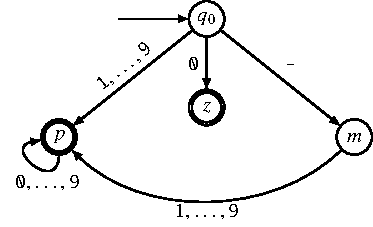
\includegraphics{3-regulaer/images/zahlennea.pdf}
\end{center}
Aus Zustand $q_0$ ist kein Übergang mit dem Zeichen {\tt 0} möglich,
dadurch werden führende Nullen verboten.
Ein {\tt -} kann nur am Anfang
stehen, befindet sich der Automat bereits im Zustand $m$ oder $p$, kann 
er keine weiteren {\tt -} akzeptieren.
Nach einem {\tt -} darf nur ein $\texttt{1}\dots\texttt{9}$ folgen,
denn vom Zustand $m$
aus gibt es keinen mit \texttt{0} angeschrieben Übergang.
\end{beispiel}

\begin{beispiel}[\bf Bedingung an ein einzelnes Zeichen]
Sei $\Sigma=\{{\tt a},{\tt b}\}$, man finde einen NEA, der die 
Sprache akzeptiert, deren Wörter an der drittletzten Stelle
eine {\tt a} haben.
Eine mögliche Lösung ist der Automat
\begin{center}
\begin{tikzpicture}[>=latex,thick]
\coordinate (q0) at (0,0);
\coordinate (q1) at (2,0);
\coordinate (q2) at (4,0);
\coordinate (q3) at (6,0);

\draw (q0) circle[radius=0.35];
\draw (q1) circle[radius=0.35];
\draw (q2) circle[radius=0.35];
\draw (q3) circle[radius=0.35];
\draw (q3) circle[radius=0.3];

\node at (q0) {$q_0$};
\node at (q1) {$q_1$};
\node at (q2) {$q_2$};
\node at (q3) {$q_3$};

\draw[->,shorten >= 0.35cm,shorten <= 0.35cm] (-2,0) -- (q0);
\draw[->,shorten >= 0.35cm,shorten <= 0.35cm] (q0) -- (q1);
\draw[->,shorten >= 0.35cm,shorten <= 0.35cm] (q1) -- (q2);
\draw[->,shorten >= 0.35cm,shorten <= 0.35cm] (q2) -- (q3);
\draw[->,shorten >= 0.35cm,shorten <= 0.35cm]
	(q0) to[out=-60,in=-120,distance=1.3cm] (q0);

\node at ($0.5*(q0)+0.5*(q1)$) [above] {\texttt{a}};
\node at ($0.5*(q1)+0.5*(q2)$) [above] {\texttt{a},\texttt{b}};
\node at ($0.5*(q2)+0.5*(q3)$) [above] {\texttt{a},\texttt{b}};
\node at ($(q0)+(0,-1)$) [below] {\texttt{a},\texttt{b}};

\end{tikzpicture}
\end{center}
Der Automat ist nicht deterministisch, weil im Zustand $q_0$ zwei verschiedene
Übergänge für das Zeichen {\tt a} möglich sind.
Der Automat bleibt
sozusagen im Zustand $q_0$ bis er ``weiss'', dass jetzt das drittletzte
Zeichen ansteht.
\end{beispiel}

\begin{beispiel}[\bf Teilbarkeit]
Für $\Sigma=\{{\tt 0}\}$ finde einen NEA für die Sprache 
\[
L=\{w\in \Sigma^*\;|\; \text{$|w|$ ist durch 2 oder 3 teilbar}\}.
\]
Das Problem bei der Konstruktion eines DEA ist, dass wird zu
Beginn noch nicht wissen können, ob wir einen ankommenden
String auf Teilbarkeit durch $2$ oder durch $3$ testen sollen.
Also verwenden wir $\varepsilon$-Übergänge aus dem Startzustand
in zwei verschiedene Automaten, die die Teilbarkeit testen:
\begin{center}
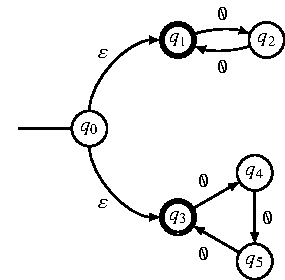
\includegraphics{3-regulaer/images/teilbarkeit.pdf}
\end{center}
\end{beispiel}

\subsection{Erreichbare Zustände\label{regulaer:erreichbarezustaende}}
\index{erreichbare Zustände}%
Im Folgenden werden wir berechnen müssen, welche Menge von Zuständen
durch einen Übergang oder mehrere verkettete Übergänge erreicht werden
können.
Es besteht ein Unterschied, ob der Übergang infolge eines
Input-Zeichens $a\in\Sigma$ erfolgt, oder ob er spontan als
$\varepsilon$-Übergang ausgeführt werden kann.

\subsubsection{Übergang zu Zeichen aus $\Sigma$}
Die Menge $\delta(q,a)\subset Q$ gibt die in einem Schritt mit Inputzeichen $a$
von $q$ aus erreichbaren Zustände von $Q$ an.
Für den Input $a_1a_2$ kann
man von jedem Zustand in $\delta(q,a_1)$ aus weiter Zustände mit einem
Überang mit Inputzeichen $a_2$ erreichen.
Die Menge der erreichbaren Zustände ist
\begin{equation}
\delta(q,a_1a_2)=\bigcup_{q_1\in\delta(q,a_1)}\delta(q_1, a_2)
=\delta(\delta(q,a_1),a_2)
\label{erreichbar}
\end{equation}
Dies kann man wiederholen:
\begin{align*}
\delta(q,a_1a_2a_3)&=
\bigcup_{q_2\in\delta(q, a_1a_2)}\delta(q_2,a_3)
=
\delta(\delta(\delta(q,a_1),a_2),a_3)
\\
\delta(q,a_1\dots a_n)&=\bigcup_{q_{n-1}\in\delta(q,a_1\dots a_{n-1})}\delta(q_{n-1},a_n)
=\delta(\dots \delta(q,a_1)\dots,a_n)
\end{align*}
Die so definierte Menge $\delta(q,a_1\dots a_n)$ umfasst alle von
$q$ aus erreichbaren Zustände.

Falls $q'\in\delta(q,a_1\dots a_n)$ gibt
es insbesondere eine Folge von Zwischenzuständen $q_1,\dots,q_{n-1}$
mit $q_k\in\delta(q_{k-1},a_k)$ für alle $k$.
Ausserdem  ist natürlich $q_k\in\delta(q,a_1\dots a_k)$ für alle $k$.

Eine Menge $M$ von Zuständen stellt man sich am besten vor, indem man die
darin enthaltenen Zustände farbig markiert.
In der Menge $\delta(M,a)$ befinden sich alle Zustände, die von Zuständen
von $M$ aus mit Input $a$ erreichbar sind.

\subsubsection{$\varepsilon$-Übergänge}
Einzelne Zustände kann man auch durch $\varepsilon$-Übergänge
erreichen.
Die Menge der Zustände, die von $q\in Q$ aus durch
$\varepsilon$-Übergänge erreichbar sind, bezeichnen wir mit
$E(q)$.
Sie setzt sich zusammen aus Zuständen, die in einem einzigen 
Schritt erreichbar sind, und solchen, die durch wiederholte
Schritte erreichbar werden.
\[
E(q)=\{q\} \cup \delta(q,\varepsilon) \cup \delta(\delta(q,\varepsilon),\varepsilon)\cup\dots
\]

\subsection{''Könnte''-Automat\label{Thompson-NEA}}
Ein NEA hat bei jedem Übergang eventuell mehrere Zielstände zur Auswahl.
Eine Implementation muss im Prinzip alle diese Möglichkeiten 
durchprobieren.
Alternativ könnte er sich aber auch merken,
welche möglichen Zustände im Laufe der Verarbeitung eines
Wortes erreicht werden konnten.
Die Menge der möglichen erreichten Zustände kann mit jedem
neuen Zeichen des Inputwortes neu berechnet werden.
Eine separate Speicherung ist nicht erforderlich, wenn man die
erreichten Zustände mit einer Markierung versieht.

\begin{figure}
\begin{center}
\includegraphics{images/reg-2}
\end{center}
\caption{Beispiel eines NEA\label{koenntenea}}
\end{figure}

\begin{figure}
\begin{center}
\begin{tabular}{cccc}
&%
\includegraphics{images/reg-2}&
\raisebox{60pt}{$\overset{\displaystyle\text{\tt b}}\longrightarrow$}&
\includegraphics{images/reg-3}\\
\raisebox{60pt}{$\overset{\displaystyle\text{\tt a}}\longrightarrow$}&
\includegraphics{images/reg-4}&
\raisebox{60pt}{$\overset{\displaystyle\text{\tt a}}\longrightarrow$}&
\includegraphics{images/reg-5}
\end{tabular}
\end{center}
\caption{Verarbeitung des Wortes {\tt baa} durch den NEA von
Abbildung~\ref{koenntenea}.
Die möglichen Zustände sind jeweils
rot markiert.\label{koenntebeispiel}
}
\end{figure}
Abbildung~\ref{koenntenea} zeigt einen NEA mit drei Zuständen.
Wir verfolgen die Verarbeitung des Wortes {\tt baa} in
Abbildung~\ref{koenntebeispiel}.

Bevor ein Zeichen verarbeitet wird,
ist der NEA im Startzustand $q_0$, also ist genau dieser Zustand
markiert.
Die Verarbeitung des Zeichens {\tt b} ist deterministisch,
sie bringt den NEA in den Zustand $q_1$.
Das folgende Zeichen {\tt a}
ist jedoch nicht mehr deterministisch, es sind sowohl $q_1$ als auch
$q_2$ als Folgezustände möglich.
Die markierte mögliche Menge von Zuständen nach Verarbeitung von {\tt ba}
ist daher $\{q_1,q_2\}$.
Bei der Verarbeitung des zweiten {\tt a} kommt noch der Zustand $q_0$ hinzu.
Man berechnet also schrittweise die
Menge der erreichbaren Zustände $\delta(q_0,{\tt baa})$.

Nach Verarbeitung des ganzen Wortes kann der NEA in den Zuständen
$\{q_0,q_1,q_2\}$ sein.
Da der Akzeptierzustand $q_0$ in dieser Menge
enthalten ist, gibt es eine Kombination von nichtdeterministischen
Entscheidungen, die zu $q_0$ führen, das Wort {\tt baa} kann also
akzeptiert werden.

\index{Thompson, Ken}%
\index{Thompson-NEA}%
Diese Implementation eines NEA geht auf Ken Thompson zurück, sie wurde in
der Regex-Library der achten Edition von Unix von Rob Pike
\index{Pike, Rob}%
implementiert, die allerdings nicht sehr weit verbreitet war.
Später hat Henry Spencer die Regex-Library neu
implementiert, allerdings ohne die Thompson-NEA Konstruktion, sondern
mit Backtracking.
Da er sie in den public domain freigab, hat sie sich
rasch verbreitet und bildete die Basis Regex-Bibliotheken in Perl, PCRE,
Python und vielen anderen.

\subsection{Transformation NEA \texorpdfstring{$\rightarrow$}{->} DEA\label{regulaer:nea-dea}}
NEAs führen trotz der beträchtlichen Erweiterung durch den
Nichtdeterminismus nicht zu einer grösseren Klasse von akzeptierbaren
Sprachen.
Dazu genügt es zu zeigen, dass sich jeder NEA in einen DEA
transformieren lässt, der die gleiche Sprache akzeptiert.
Dass dies möglich sein sollte, deutet bereits die Konstruktion
des Thompson-NEA in \ref{Thompson-NEA} an.
Der Thompson-NEA wird zu einem DEA, wenn man die Verteilung der
``roten Markierungen'' als Zustand des DEA ansieht.
Ziel dieses Abschnittes ist, dies
mathematisch streng zu formalisieren.

Ein NEA kann aus zwei Gründen kein DEA sein:
er kann $\varepsilon$-Übergänge haben und er kann nicht eindeutige
oder nicht existierende Übergänge haben, also $|\delta(q,a)|\ne 1$
für gewisse $q\in Q$ und $a\in\Sigma$.
Wir transformieren einen 
beliebigen NEA in zwei Schritten in einen DEA:
\begin{enumerate}
\item Wir bauen uns einen Algorithmus, mit dem man einen NEA ohne
$\varepsilon$-Übergänge in einen DEA umwandeln kann.
\item Wir modifizieren den Algorithmus, so dass er auch mit NEAs mit
$\varepsilon$-Übergängen umgehen kann.
\end{enumerate}

\subsubsection{Transformation für NEA ohne $\varepsilon$-Übergänge}
Der konstruierte DEA muss darüber Buch führen, in welchen Zuständen
der NEA sein könnte.
Seine Zustände sind als Mengen von möglichen Zuständen des NEA.
Als Zustandsmenge des DEA wird man also $P(Q)$ 
erwarten.
Wie die übrigen Elemente des DEA konstruiert werden müssen,
besagt der folgende Satz.

\begin{satz}
\label{satz_neadea_eps}
Sei $A=(Q,\Sigma,\delta,q_0,F)$ ein NEA ohne $\varepsilon$-Übergänge.
Dann gibt es einen DEA $A'$, der die gleiche Sprache akzeptiert: $L(A)=L(A')$.
Der DEA $A'$ setzt sich zusammen aus
\[
A'=
(P(Q), \Sigma, \delta', \{q_0\}, F'),
\]
die Übergangsfunktion ist
\[
\delta'\colon P(Q)\times \Sigma: (M, a)\mapsto \bigcup_{q\in M} \delta(q,a)
=\delta(M,a),
\]
und die Akzeptierzustände sind die Teilmengen, die einen Akzeptierzustand
enthalten:
\[
F'=\{M\in P(Q)\;|\;M\cap F\ne \emptyset\}.
\]
\end{satz}
\begin{proof}[Beweis]
Es ist klar, dass mit dieser Übergangsfunktion $\delta'$ und den
Akzeptierzuständen $F'$ ein DEA definiert ist, es muss nur noch
bewiesen werden, dass er die gleiche Sprache akzeptiert, also
$L(A)=L(A')$.
Das wird zutreffen, wenn $L(A)\subset L(A')$ und
$L(A')\subset L(A)$, also jedes Wort von $L(A)$ ist auch in $L(A')$,
und umgekehrt.

Wenn $w=a_1\dots a_n\in L(A)$, dann gibt es einen Pfad durch den gerichteten
Graphen von $A$, der zu einem Akzeptierzustand führt.
Also enthält
die Menge der von $q_0$ aus erreichbaren Zustände einen Akzeptierzustand.
Diese Menge ist aber die Menge der Zustände, die man durch Anwendung
von $\delta'$ aus $\{q_0\}$ und den Inputzeichen $a_1,\dots,a_n$ erhalten
wird.
Da diese Menge einen Akzeptierzustand enthält, ist sie ein
Akzeptierzustand von $A'$ und damit $w\in L(A')$.

Sei jetzt umgekehrt $w\in L(A')$.
Wir schreiben wieder $w=a_1\dots a_n$.
Auf Grund der Konstruktion des Automaten $A'$, liefert die wiederholte
Anwendung von $\delta'(\cdot, a_k)$ aus dem Anfangszustand $q_0'=\{q_0\}$
die Menge $\delta(\dots\delta(q_0, a_1)\dots ,a_n)$.
Da diese Menge ein
Akzeptierzustand von $A'$ ist, gibt es darin einen Akzeptierzustand
von $A$.
Da also ein Akzeptierzustand erreichbar ist, ist $w\in L(A)$,
also auch $L(A')\subset L(A)$.
\end{proof}

\subsubsection{Beispiel}
Der NEA von Abbildung~\ref{koenntenea}
%\[
%\entrymodifiers={++[o][F]}
%\xymatrix{
%*+\txt{}\ar[r]
%	&*++[o][F=]{q_0} \ar[d]_{\tt b} 
%		&{q_2}\ar[l]_{\tt a}
%\\
%*+\txt{}
%	&{q_1}\ar[ur]_{{\tt a},{\tt b}} \ar@(ul,dl)_{\tt a}
%}
%\]
soll in einen DEA umgewandelt werden.
Er ist nicht deterministisch,
weil vom Zustand $q_1$ aus zwei Übergänge mit {\tt a} möglich sind.

Aus dem Satz ist bekannt, dass die Zustände die Potenzmengen von $Q$ sind.
Diese entsprechen den dreistelligen Binärzahlen, wobei jede
Stelle angibt, ob das zugehörige $q_i$ in der Menge dabei ist.
Wir
schreiben also
\begin{align*}
       &          &q_{001}&=\{\phantom{q_2q_1}q_0\}&q_{110}&=\{q_2,q_1\phantom{,q_0}\}&&\\
q_{000}&=\emptyset&q_{010}&=\{\phantom{q_2}q_1\phantom{q_0}\}&q_{101}&=\{q_2,\phantom{q_1,}q_0\}&q_{111}&=\{q_2,q_1,q_0\}\\
       &          &q_{100}&=\{q_2\phantom{q_1q_0}\}&q_{011}&=\{\phantom{q_2,}q_1,q_0\}&&\\
\end{align*}
Akzeptierzustände sind jene Mengen, die $q_0$ enthalten, also
\[
F'=\{ q_{001}, q_{011}, q_{101}, q_{111}\},
\]
Startzustand ist $q_{001}$.
Damit können wir jetzt das Zustandsdiagramm zeichnen
\[
\entrymodifiers={++[o][F]}
\xymatrix{
*+\txt{}\ar[r]
	&*++[o][F=]{q_{001}} \ar[d]^{\tt b}\ar[dl]_{\tt a}
		&{q_{110}}\ar[dr]^{\tt a} \ar[ddl]^{\tt b}
\\
{q_{000}}\ar@(ul,dl)_{{\tt a},{\tt b}}
	&{q_{010}} \ar[ur]^{\tt a} \ar[d]^{\tt b}
		&*++[o][F=]{q_{101}} \ar[ul]^{\tt a} \ar[l]^{\tt b}
			&*++[o][F=]{q_{111}}\ar@(ur,dr)^{{\tt a}} \ar@/_20pt/[ul]_{\tt b}
\\
*+\txt{}
	&{q_{100}}\ar@/^20pt/[uu]^{\tt a}  \ar[ul]^{\tt b}
		&*++[o][F=]{q_{011}} \ar@/_20pt/[uu]_{{\tt a},{\tt b}}
}
\]
Man erkennt sofort, dass die Zustände $q_{101}$ und $q_{011}$
nicht erreicht werden können, also weggelassen werden könnten:
\begin{equation}
\entrymodifiers={++[o][F]}
\xymatrix{
*+\txt{}\ar[r]
	&*++[o][F=]{q_{001}} \ar[d]^{\tt b}\ar[dl]_{\tt a}
		&{q_{110}}\ar[dr]^{\tt a} \ar[ddl]^{\tt b}
\\
{q_{000}}\ar@(ul,dl)_{{\tt a},{\tt b}}
	&{q_{010}} \ar[ur]^{\tt a} \ar[d]^{\tt b}
		&*+\txt{}
			&*++[o][F=]{q_{111}}\ar@(ur,dr)^{{\tt a}} \ar@/_20pt/[ul]_{\tt b}
\\
*+\txt{}
	&{q_{100}}\ar@/^20pt/[uu]^{\tt a}  \ar[ul]^{\tt b}
		&*+\txt{}
}
\label{nea-eps}
\end{equation}
Man kann ebenfalls verifzieren, dass dies tatsächlich ein DEA ist, 
von jedem Zustand gehen genau zwei Pfeile für die Übergänge mit
den Zeichen ${\tt a}$ und ${\tt b}$ aus.
Etwas übersichtlicher geschrieben lautet er
\[
\entrymodifiers={++[o][F]}
\xymatrix{
*+\txt{}\ar[r]
	&*++[o][F=]{1}\ar[r]^{\tt b} \ar[d]_{\tt a}
		&2 \ar[r]^{\tt a} \ar[d]^{\tt b}
			&6\ar@/_/[r]_{\tt a} \ar[dl]^{\tt b}
				&*++[o][F=]{7}\ar@/_/[l]_{\tt b} \ar@(ur,dr)^{\tt a}
\\
*+\txt{}
	&0 \ar@(l,d)_{{\tt a},{\tt b}}
		&4 \ar[ul]_{\tt a} \ar[l]^{\tt b}
}
\]

\subsubsection{NEA mit $\varepsilon$-Übergängen}
Wir erweitern die Konstruktion des DEA aus einem NEA jetzt, um eventuell
vorhandenen $\varepsilon$-Übergängen Rechnung zu tragen.

\begin{satz}
\label{satz_neadea}
Sei $A=(Q,\Sigma,\delta,q_0,F)$ ein NEA, dann gibt es einen
DEA $A'=(Q',\Sigma,\delta',q_0',F')$, der die gleiche Sprache
akzeptiert, $L(A)=L(A')$.
Es ist
\begin{align*}
Q'&=P(Q)\\
\delta'(M,a)&=E(\delta(M, a))\quad M\in P(Q)\\
q_0'&=E(q_0)\\
F'&=\{M\in P(Q)\;|\, M\cap F\ne \emptyset\}
\end{align*}
\end{satz}

\begin{proof}[Beweis]
Gegenüber Satz \ref{satz_neadea} hat sich geändert, dass wir den
Anfangszustand von $\{q_0\}$ auf $E(q_0)$ vergrössert haben.
Dadurch erfassen wir alle Pfade durch den Automaten, die mit einem oder
mehreren $\varepsilon$-Übergängen beginnen.
Falls $E(q_0)\cap F\ne \emptyset$
wird der Anfangszustand auch zu einem Endzustand.

Zudem erweitern wir in der Definition des Bildes $\delta(M,a)$ um alle Zustände,
die durch einen angehängten $\varepsilon$-Übergang erreicht werden
können.
\end{proof}

\subsubsection{Beispiel}
Der NEA 
\[
\entrymodifiers={++[o][F]}
\xymatrix{
*+\txt{}\ar[r]
	&*++[o][F=]{q_0} \ar[d]_{\tt b} \ar@/_/[r]_{\varepsilon}
		&{q_2}\ar@/_/[l]_{\tt a}
\\
*+\txt{}
	&{q_1}\ar[ur]_{{\tt a},{\tt b}} \ar@(ul,dl)_{\tt a}
}
\]
soll in einen DEA umgewandelt werden.

Den NEA ohne den $\varepsilon$-Übergang haben wir bereits in
\ref{nea-eps} umgewandelt.
Jetzt müssen wir nur die beiden
im Satz \ref{satz_neadea} erwähnten Modifikationen durchführen.

Ursprünglich war der Startzustand $q_{001}$.
Da aus dem Startzustand
des NEA mittels $\varepsilon$-Übergang auch der Zustand $q_2$
erreichbar ist, muss der Anfangszustand des DEA um diesen Zustand
erweitert werden und ist jetzt $q_{101}$:
\[
\entrymodifiers={++[o][F]}
\xymatrix{
*+\txt{}
	&*++[o][F=]{q_{001}} \ar[d]^{\tt b}\ar[dl]_{\tt a}
		&{q_{110}}\ar[dr]^{\tt a} \ar[ddl]^{\tt b}
\\
{q_{000}}\ar@(ul,dl)_{{\tt a},{\tt b}}
	&{q_{010}} \ar[ur]^{\tt a} \ar[d]^{\tt b}
		&*++[o][F=]{q_{101}} \ar[ul]^{\tt a} \ar[l]^{\tt b}
			&*++[o][F=]{q_{111}}\ar@(ur,dr)^{{\tt a}} \ar@/_20pt/[ul]_{\tt b}
\\
*+\txt{}
	&{q_{100}}\ar@/^20pt/[uu]^{\tt a} \ar[ul]^{\tt b}
		&*++[o][F=]{q_{011}} \ar@/_20pt/[uu]_{{\tt a},{\tt b}}
			&*+\txt{}\ar[ul]
}
\]


Zusätzlich müssen wir bei jedem Übergang die Möglichkeit in
Betracht ziehen, dass noch ein $\varepsilon$-Übergang angehängt
wird.
Dies bedeutet im vorliegenden Fall, dass bei jedem Übergang,
der zu einem $q_0$ enthaltenden Zustand führt, auch noch der
Zustand $q_2$ hinzugefügt werden muss.
\[
\entrymodifiers={++[o][F]}
\xymatrix{
*+\txt{}
	&*++[o][F=]{q_{001}} \ar[d]^{\tt b}\ar[dl]_{\tt a}
		&{q_{110}}\ar[dr]^{\tt a} \ar[ddl]^{\tt b}
\\
{q_{000}}\ar@(ul,dl)_{{\tt a},{\tt b}}
	&{q_{010}} \ar[ur]^{\tt a} \ar[d]^{\tt b}
		&*++[o][F=]{q_{101}} \ar@(ul,ur)^{\tt a} \ar[l]^{\tt b}
			&*++[o][F=]{q_{111}}\ar@(ur,dr)^{{\tt a}} \ar@/_20pt/[ul]_{\tt b}
\\
*+\txt{}
	&{q_{100}}\ar[ur]^{\tt a} \ar[ul]^{\tt b}
		&*++[o][F=]{q_{011}} \ar@/_20pt/[uu]_{{\tt a},{\tt b}}
			&*+\txt{}\ar[ul]
}
\]
In diesem Automaten sind die Zustände $q_{001}$ und $q_{011}$ nicht
mehr erreichbar, man kann sie weglassen.
\[
\entrymodifiers={++[o][F]}
\xymatrix{
*+\txt{}
	&*+\txt{}
		&{q_{110}}\ar[dr]^{\tt a} \ar[ddl]^{\tt b}
\\
{q_{000}}\ar@(ur,dr)^{{\tt a},{\tt b}}
	&{q_{010}} \ar[ur]^{\tt a} \ar[d]^{\tt b}
		&*++[o][F=]{q_{101}} \ar@(ul,ur)^{\tt a} \ar[l]^{\tt b}
			&*++[o][F=]{q_{111}}\ar@(ur,dr)^{{\tt a}} \ar@/_20pt/[ul]_{\tt b}
\\
*+\txt{}
	&{q_{100}}\ar[ur]^{\tt a} \ar[ul]^{\tt b}
		&*+\txt{}
			&*+\txt{}\ar[ul]
}
\]
Wie man mit dem Algorithmus über den Minimalautomaten kontrollieren
kann, lässt sich dieser Automat nicht mehr weiter reduzieren.
Etwas übersichtlicher geschrieben lautet er
\[
\entrymodifiers={++[o][F]}
\xymatrix{
*+\txt{}\ar[r]
	&*++[o][F=]{5}\ar@(ul,ur)^{\tt a} \ar[r]^{\tt b}
		&2\ar[r]^{\tt a} \ar[d]^{\tt b}
			&6\ar@/_/[r]_{\tt a} \ar[dl]^{\tt b}
				&*++[o][F=]{7}\ar@/_/[l]_{\tt b} \ar@(ur,dr)^{\tt a}
\\
*+\txt{}
	&0\ar@(ul,dl)_{{\tt a},{\tt b}}
		&4\ar[ul]^{\tt a} \ar[l]^{\tt b}
}
\]


Satz \ref{satz_neadea} ist nicht nur ein theoretisch interessantes
Resultat.
Wenn man die endliche vielen Zustände mit den Zahlen
$0,\dots,|Q|-1$ identifiziert, kann man die Teilmengen von $Q$ mit
den $|Q|$-stelligen Binärzahlen identifizieren.
Der Teilmenge $M\subset Q$ entsprechen die Binärzahlen, die Einsen an
den Stellen haben, deren Nummern in $M$ enthalten sind.
Die grosse Vereinigungen ist ebenfalls sehr einfach
zu berechnen, sie entspricht der Oder-Verknüpfung
der einzelnen Mengen in (\ref{erreichbar}).
Somit haben wir nicht nur ein Existenz-Resultat, sondern einen
Algorithmus, mit dem ein beliebiger NEA in einen DEA umgewandelt
werden kann.
Daraus können wir jetzt einen Vergleichsalgorithmus für reguläre
Sprachen ableiten: 

\begin{satz}
Es gibt einen Algorithmus, mit dem entschieden werden kann, ob
zwei Automaten $A$ und $B$ die gleiche Sprache akzeptieren.
\end{satz}

\begin{proof}[Beweis]
Um zu entscheiden, ob $L(A)=L(B)$, wendet man folgenden Algorithmus
an:
\begin{enumerate}
\item Wandle $A$ und $B$
mit dem Algorithmus des Satzes 
\ref{satz_neadea} in die DEAs $A'$ und $B'$ um.
\item Reduziert anschliessend $A'$ und $B'$  mit dem Algorithmus
von Satz \ref{satz_minimalautomat} in Minimalautomaten
$A''$ und $B''$.
\item Die von $A$ und $B$ akzeptierten Sprachen sind genau dann
gleich, wenn $A''$ und $B''$ identisch sind.
\end{enumerate}
\end{proof}

Der hier vorgeschlagene Beweis ist allerdings oft nicht praktikabel.
Der aus dem NEA erzeugte DEA hat im schlechtesten Fall $2^n$
Zustände, wenn der NEA $n$ Zustände hatte, die Laufzeit des
Algorithmus ist also exponentiell in der Grösse des NEA.
Ein wesentlich schnellerer Algorithmus wurde 2015 von Bonchi und Pous
gefunden \cite{skript:bonchi-pous}.

\subsection{Mengenoperationen\label{regulaer:mengenoperationen}}
\index{Mengenoperationen}%
\index{Durchschnitt}%
\index{Vereinigung}%
\index{Differenz}%
Sprachen sind Mengen von Wörtern, also sind auch deren Vereinigung,
Durchschnitt, Differenz usw.~Sprachen.
Sind die Sprachen regulär,
sind dann auch Vereinigung, Durchschnitt, Differenz etc.~regulär? 
NEAs erlauben uns sehr elegant zu zeigen, dass Sie diese Operationen
alle wieder reguläre Sprachen liefern.

\begin{satz}
\index{Vereinigung}%
\label{satz_union}
Sind $L_1$ und $L_2$ reguläre Sprachen, dann
ist auch $L_1\cup L_2$ regulär.
\end{satz}

\begin{figure}
\begin{center}
\includegraphics{images/nea-5}
\qquad \qquad
\includegraphics{images/nea-6}
\end{center}
\caption{Konstruktion eines NEA 
für die Sprache $L(A_1)\cup L(A_2)$.\label{regulaer:vereinigung}}
\end{figure}

\begin{proof}[Beweis]
Da die Sprachen regulär sind, gibt es endliche Automaten 
\begin{align*}
A_1&=(Q_1,\Sigma_1,\delta_1, q_{01}, F_1)\\
A_2&=(Q_2,\Sigma_2,\delta_2, q_{02}, F_2)
\end{align*}
mit $L_1=L(A_1)$ und $L_2=L(A_2)$.
Wir müssen
jetzt einen Automaten
\[
A = (Q, \Sigma, \delta, q_0, F)
\]
konstruieren, der $L_1\cup L_2$ akzeptieren
(Abbildung~\ref{regulaer:vereinigung}).

Für die Vereinigung muss das Alphabet alle Zeichen enthalten,
also $\Sigma = \Sigma_1\cup\Sigma_2$.
Man kann jeden der Automaten 
$A_1$ und $A_2$ auch als Automaten über dem Alphabet $\Sigma$
betrachten, indem man setzt
\[
\delta_i(q, x)=\begin{cases}
\delta_i(q,x)&\qquad q\in Q_i\text{ und } x\in \Sigma_i\\
\emptyset&\qquad q\in Q_i\text{ und } x\in \Sigma_{3-i}\setminus \Sigma_i\\
\end{cases}
\]
Es ist also keine Einschränkung, wenn wir annehmen, dass
$\Sigma=\Sigma_1=\Sigma_2$.

Um den Automaten für $L_1\cup L_2$ zu konstruieren, nehmen wir jetzt
weiter an, dass $Q_1$ und $Q_2$ disjunkt sind.
Für $A$ verwenden wir einen neuen Startzustand $q_0$.
Ein Wort in $L_1\cup L_2$ muss von einem der beiden Automaten
akzeptiert werden.
Der Automat muss sich also zu Beginn nichtdeterministisch
dafür entscheiden, den einen oder anderen Automaten zum
akzeptieren eines Wortes zu verwenden.
Also verwenden wir 
\begin{align*}
Q&=Q_1\cup Q_2\cup \{q_0\}\\
F&=F_1\cup F_2\\
\delta(x,a)&=\begin{cases}
\delta_1(x,a)&\qquad x\in Q_1\\
\delta_2(x,a)&\qquad x\in Q_2\\
\{q_{01}, q_{02}\}&\qquad x=q_0, a=\varepsilon\\
\emptyset&\qquad x=q_0, a\ne\varepsilon
\end{cases}
\end{align*}
\end{proof}

\begin{satz}
\index{Durchschnitt}%
\label{satz_intersection}
Sind $L_1$ und $L_2$ reguläre Sprachen, dann
ist auch $L_1\cap L_2$ regulär.
\end{satz}

\begin{proof}[Beweis]
Da die Sprachen regulär sind, gibt es endliche Automaten 
\begin{align*}
A_1&=(Q_1,\Sigma_1,\delta_1, q_{01}, F_1)\\
A_2&=(Q_2,\Sigma_2,\delta_2, q_{02}, F_2)
\end{align*}
mit $L_1=L(A_1)$ und $L_2=L(A_2)$.
Wir müssen jetzt einen Automaten
\[
A = (Q, \Sigma, \delta, q_0, F)
\]
konstruieren, der $L_1\cap L_2$ akzeptiert.

Für die Schnittmenge brauchen wir einen Automaten, der die Abläufe 
in beiden Teilautomaten gleichzeitig codiert.
Dies ist möglich, indem man Zustände und Übergänge nebeneinander
simuliert.
Als Zustandsmenge verwenden wir daher $Q=Q_1\times Q_2$.
Als Übergangsfunktion verwenden wir
\[
\delta((q',q''),a)=\delta_1(q',a)\times \delta_2(q'',a).
\]
Akzeptiert werden kann ein Wort, wenn beide Komponenten des Paares 
Akzeptierzustände ihrer Automaten sind.
Akzeptierzustände von $A$ sind also $F=F_1\times F_2$.
\end{proof}

\index{Produktautomat}%
Wir nennen diesen mit Hilfe des kartesischen Produktes konstruierten
Automaten auch den
{\em kartesischen Produktautomaten}\label{reg_produktautomat}.

\subsubsection{Beispiel}
Zur Illustration wollen 
wir einen Automaten für die Schnittmenge von
\begin{align*}
L_1&=\{w\in\Sigma^*\;|\; \text{$|w|_0$ gerade}\}\qquad\text{und}\\
L_2&=\{w\in\Sigma^*\;|\,\text{$w$ ist eine durch 3 teilbare Binärzahl}\}.
\end{align*}
konstruieren.
Die einzelnen Teilautomaten sind $A_1$ für $L_1$:
\[
\entrymodifiers={++[o][F]}
\xymatrix{
*+\txt{}\ar[r]
	&*++[o][F=]{} \ar@/^/[r]^{\tt 0} \ar@(ul,ur)^{\tt 1}
		&{} \ar@/^/[l]^{\tt 0} \ar@(ul,ur)^{\tt 1}
}
\]
und $A_2$ für $L_2$
\[
\entrymodifiers={++[o][F]}
\xymatrix{
*+\txt{}\ar[r]
	&*++[o][F=]{0} \ar@/^/[r]^{\tt 1} \ar@(ul,ur)^{\tt 0}
		&{1} \ar@/^/[l]^{\tt 1} \ar@/^/[r]^{\tt 0}
			&{2}\ar@(ur,dr)^{\tt 1} \ar@/^/[l]^{\tt 0}
}
\]
Der Produktautomat ist jetzt
\[
\entrymodifiers={++[o][F]}
\xymatrix{
*+\txt{} \ar[r] \ar[d] \ar[dr]
	&*++[o][F=]{0} \ar@/^/[r]_{\tt 1} \ar@(ul,ur)^{\tt 0}
		&{1} \ar@/^/[l] \ar@/^/[r]_{\tt 0}
			&{2}\ar@(ur,dr)^{\tt 1} \ar@/^/[l]
\\
*++[o][F=]{} \ar@/^/[d] \ar@(ul,dl)_{\tt 1}
	&*++[o][F=]{} \ar@/^/[d]{\tt 0} \ar@/^/[r]_{\tt 1}
		&{} \ar@/^/[l] \ar@/^/[dr]_{\tt 0}
			&{}\ar@(ur,dr)^{\tt 1} \ar@/^/[dl]
\\
{} \ar@/^/[u]_{\tt 0} \ar@(ul,dl)_{\tt 1}
	&{} \ar@/^/[u]_{\tt 0} \ar@/^/[r]_{\tt 1}
		&{} \ar@/^/[l] \ar@/^/[ur]
			&{}\ar@(ur,dr)^{\tt 1} \ar@/^/[ul]
}
\]

Man kann den Produktautomaten auch
verwenden, um einen Automaten zu bauen, der $L_1\cup L_2$
akzeptiert.
Der kartesische Produktautomat simuliert ja sozusagen
beide Teilautomaten in den beiden Komponenten der Zustände.
Akzeptabel ist ein Wort $w$, wenn es von $A_1$
oder von $A_2$ akzeptiert ist, oder wenn der Produktautomat
sich am Ende des Wortes in einem Zustand befindet, der ein
Akzeptierzustand von $A_1$ ist oder von $A_2$.
Verwendet
man also $F_1\times Q_2\cup Q_1\times F_2$ als Akzeptierzustände,
erhält man einen Automaten, der $L_1\cup L_2$ akzeptiert.
Das zugehörige Zustandsdiagramm ist:
\[
\entrymodifiers={++[o][F]}
\xymatrix{
*+\txt{} \ar[r] \ar[d] \ar[dr]
	&*++[o][F=]{0} \ar@/^/[r]_{\tt 1} \ar@(ul,ur)^{\tt 0}
		&{1} \ar@/^/[l] \ar@/^/[r]_{\tt 0}
			&{2}\ar@(ur,dr)^{\tt 1} \ar@/^/[l]
\\
*++[o][F=]{} \ar@/^/[d] \ar@(ul,dl)_{\tt 1}
	&*++[o][F=]{} \ar@/^/[d]{\tt 0} \ar@/^/[r]_{\tt 1}
		&*++[o][F=]{} \ar@/^/[l] \ar@/^/[dr]_{\tt 0}
			&*++[o][F=]{}\ar@(ur,dr)^{\tt 1} \ar@/^/[dl]
\\
{} \ar@/^/[u]_{\tt 0} \ar@(ul,dl)_{\tt 1}
	&*++[o][F=]{} \ar@/^/[u]_{\tt 0} \ar@/^/[r]_{\tt 1}
		&{} \ar@/^/[l] \ar@/^/[ur]
			&{}\ar@(ur,dr)^{\tt 1} \ar@/^/[ul]
}
\]

\begin{satz}
\index{Differenz}%
\label{satz_regcomplement}
Ist $L$ eine reguläre Sprache, dann ist auch $\bar L$ regulär.
Sind $L_1$ und $L_2$ regulär, dann ist auch $L_1\setminus L_2$
regulär.
\end{satz}

\begin{proof}[Beweis]
Da $L$ regulär ist, gibt es einen DEA, welcher $L=L(A)$ erfüllt.
Wir ersetzen in diesem DEA die Menge $F$ der Akzeptierzustände
durch $Q\setminus F$ und erhalten einen neuen DEA $A'$.
Dieser neue DEA akzeptiert genau diejenigen Wörter, die $A$ nicht
akzeptiert hat, also $L(A')=\overline{L(A)}$.
Somit ist $\bar L=L(A')$ regulär.

Die zweite Aussage folgt aus $L_1\setminus L_2=L_1\cap\bar L_2$ und
Satz \ref{satz_intersection}
\end{proof}
Man beachte, dass in diesem Beweis unbedingt ein DEA verwendet werden
muss.
Die beiden NEAs
\[
\entrymodifiers={++[o][F]}
\xymatrix{
*+\txt{}\ar[r]
	&{}\ar@(ul,ur)^{\Sigma} \ar[r]^{\varepsilon}
		&*++[o][F=]{}
&
*+\txt{}\ar[r]
	&*++[o][F=]{}\ar@(ul,ur)^{\Sigma} \ar[r]^{\varepsilon}
		&{}
}
\]
gehen auseinander durch Ersetzung der Akzeptierzustände
$F\leftrightarrow Q\setminus F$ hervor, aber beide akzeptieren
$\Sigma^*$, also nicht das Komplement.


\rhead{Reguläre Ausdrücke}
\section{Reguläre Ausdrücke\label{regulaer:re}}
\index{reguläre Ausdrücke}%
Endliche Automaten beschreiben reguläre Sprachen, sind aber für die
Anwendung eher unhandlich.
In der Praxis haben sich reguläre Ausdrücke
durchgesetzt, die mit einer einfachen Syntax ebenfalls Mengen von
Wörtern zu spezifizieren erlauben.
Ziel dieses Abschnittes ist
zu zeigen, dass reguläre Ausdrücke genau gleich ausdrucksstark sind
wie DEAs.

\subsection{Reguläre Operationen\label{regulaer:regulaere-operationen}}
\index{reguläre Operationen}%
Wir wissen bereits, dass wir die Mengenoperationen auf reguläre
Sprachen anwenden dürfen, ohne die Klasse der regulären Sprachen
zu verlassen.
Es sind jedoch noch zwei weitere Operationen möglich, die ebenfalls
nicht aus der Klasse herausführen:

\begin{definition}
\index{Verkettung}%
Seien $L_1$ und $L_2$ Sprachen, dann ist die
Verkettung von $L_1$ und $L_2$ die Sprache
\[
L_1L_2=\{w_1w_2\;|\;w_1\in L_1,w_2\in L_2\}.
\]
Die mehrfache Verkettung von $L$ wird mit $L^n$ bezeichnet:
\begin{align*}
L^0&=\{\varepsilon\}\\
L^n&=L^{n-1}L
\end{align*}
\end{definition}

\begin{definition}
\index{*-Operation@$*$-Operation}%
Sei $L$ eine Sprache, dann ist die Stern-Operation
von $L$ die Sprache
\[
L^*=\bigcup_{k\in\mathbb N} L^k.
\]
\end{definition}

Wir möchten jetzt zeigen, dass diese Operationen nicht aus den
regulären Sprachen herausführen.
Dazu müssen wir zu gegebenen Automaten $A_1$ und $A_2$ für zwei Sprachen
$L_1$ und $L_2$ neue Automaten konstruieren, welche
die Sprachen $L_1L_2$ oder $L_1^*$ akzeptieren.
Die Automaten $A_1$ und $A_2$ müssen wir dabei als ``Black Box'' betrachten,
wir dürfen daran nichts ändern.

\subsubsection{Automat zu einer Verkettung $L_1L_2$}
\index{Verkettung}%
Für die Verkettung $L_1L_2$ ist es zum Beispiel
nicht zulässig, die Akzeptierzustände von
$A_1$ mit dem Startzustand von $A_2$ zusammenzulegen.
Dadurch
würde es nämlich möglich, auch Wege wieder zurück in
den ersten Automaten zu verwenden.
Im folgenden Beispiel akzeptiert der erste Automat Strings mit
einer ungeraden Anzahl Nullen, der zweite Strings mit einer
ungeraden Anzahl {\tt a}.
\[
\entrymodifiers={++[o][F]}
\xymatrix{
*+\txt{}\ar[r]
	&{} \ar@/^/[r]^{\tt 0}
		&*++[o][F=]{} \ar@/^/[l]^{\tt 0}
			&*\txt{}\ar[r]
				&{} \ar@/^/[r]^{\tt a}
					&*++[o][F=]{} \ar@/^/[l]^{\tt a }
}
\]
Verkettet man die Automaten, indem man den Akzeptierzustand des
ersten mit dem Startzustand des zweiten Automaten zusammenlegt,
erhält man
\[
\entrymodifiers={++[o][F]}
\xymatrix{
*+\txt{}\ar[r]
	&{} \ar@/^/[r]^{\tt 0}
		&{} \ar@/^/[l]^{\tt 0}
				 \ar@/^/[r]^{\tt a}
					&*++[o][F=]{} \ar@/^/[l]^{\tt a }
}
\]
Dieser Automat akzeptiert aber auch das Wort {\tt 0aa00a}, welches
gar nicht in $L_1L_2$ ist! Die Verkettung muss also mit Hilfe
einer ``Einbahnstrasse'' erfolgen, ein $\varepsilon$-Übergang
ist ideal dafür geeignet.
Die folgende Verkettung funktioniert:
\[
\entrymodifiers={++[o][F]}
\xymatrix{
*+\txt{}\ar[r]
	&{} \ar@/^/[r]^{\tt 0}
		&{} \ar@/^/[l]^{\tt 0} \ar[r]^{\varepsilon}
			&{} \ar@/^/[r]^{\tt a}
				&*++[o][F=]{} \ar@/^/[l]^{\tt a }
}
\]

Für die allgemeine Konstruktion gehen wir aus
von zwei Automaten $A_1$ und $A_2$:
\begin{center}
\includegraphics{images/nea-1}
\end{center}
Ein Automat für die Verkettung entsteht, indem man
die Akzeptierzustände im ersten Automaten über
$\varepsilon$-Übergänge mit dem
Startzustand des zweiten verbindet:
\begin{center}
\includegraphics{images/nea-2}
\end{center}
Die $\varepsilon$-Übergänge
fungieren als Einbahnstrassen und stellen sicher, auch innerhalb der
einzelnen Automaten keine neuen akzeptierten Wörter entstehen können.

Etwas formeller kann man das Resultat im folgenden Satz zusammenfassen.

\begin{satz}
\index{Verkettung}%
\label{satz_concat}
Sind $L_1$ und $L_2$ reguläre Sprachen, dann ist auch $L_1L_2$
regulär.
\end{satz}

\begin{proof}[Beweis]
Ein Wort $w\in L_1L_2$ besteht aus zwei Teilen, die von $L_1$
bzw.~$L_2$ akzeptiert werden.
Ein Automat $A$ für $L=L_1L_2$ kann aus Automaten $A_1$ und $A_2$
konstruiert werden, indem man
die Akzeptierzustände von $A_1$ über $\varepsilon$-Übergänge
mit dem Startzustand von $A_2$ verbindet.
Also verwenden wir $Q=Q_1\cup Q_2$.
Startzustand ist der Startzustand $q_{01}$ von $L_1$, Akzeptierzustände
sind die Akzeptierzustände $F_2$ von $A_2$.
Also
\begin{align*}
Q&=Q_1\cup Q_2\\
F&=F_2\\
q_0&=q_{01}\\
\delta(q,a)&=\begin{cases}
\delta_1(\varepsilon,a)\cup\{q_{02}\}&\qquad q\in F_1 \wedge a=\varepsilon\\
\delta_1(q,a)                        &\qquad q\in F_1 \wedge a\ne\varepsilon
\quad\text{oder}\quad q\in Q_1\setminus F_1\\
%\\
%\delta_1(q,a)                        &\qquad q\in Q_1\setminus F_1\\
\delta_2(q,a)                        &\qquad q\in Q_2
\end{cases}
\end{align*}
\end{proof}

\subsubsection{Automat zur *-Operation $L^*$}
\index{*-Operation@$*$-Operation}%
Die Stern-Operation verlangt, dass man einen Automaten mehrfach
durchlaufen können muss.
Dies könnte man mit einem $\varepsilon$-Übergang
von den Akzeptierzuständen direkt zum Startzustand realisieren.
Dadurch ändert man aber den Automaten für die Sprache $L$,
der Automat ist nicht mehr eine wiederverwendbare Einheit.

Wir streben an, die regulären Operationen ohne interne Änderungen
des Automaten zu konstruieren.
Insbesondere dürfen dem Automaten keine neuen Übergänge hinzugefügt
werden.
Es ist hingegen zulässig, einen Akzeptierzustand zu einem
Nichtakzeptierzustand zu degradieren.
Ob nämlich ein Zustand als Akzeptierzustand interpretiert wird,
hängt davon ab, was ein zusammengesetzter Automat mit der Information
macht, dass ein Teilautomat sich in einem Akzeptierzustand befindet.

Zur Verdeutlichung stelle man sich eine Automaten-Objekt $A$ vor mit
folgendem Interface
\begin{verbatim}
interface Automat {
        // Zeichen verarbeiten
        void    process(char zeichen);
        // testen, ob sich der Automat in einem Akzeptierzustand befindet
        boolean accept();
        // in den Startzustand zurueckversetzen
        void    reset();
}
\end{verbatim}
Offensichtlich enthält dieses Interface keine Möglichkeit, den Automaten
zu modifizieren, oder auch nur den inneren Zustand auf eine andere Art
zu ändern als mit einem normalen Übergang.
Das Interface genügt aber, um die *-Operation auszuführen.
Um ein Wort in $L^*$ zu akzeptieren, muss man nur jedes Zeichen
des Wortes in den Automaten $A$ einspeisen und fragen, ob er sich
in einem Akzeptierzustand befindet.
Falls ja, darf man das Teilwort
akzeptieren und den Automaten in den Startzustand zurückversetzen.

Für die *-Operation darf also der Automat
\begin{center}
\includegraphics{images/nea-3}
\end{center}
nicht modifiziert werden, insbesondere darf der naheligende
$\varepsilon$-Übergang von einem Akzeptierzustand zum Startzustand
nicht hinzugefügt werden.
Um das leere Wort muss daher ein zusätzlicher Zustand hinzugefügt werden.
Und für die Wiederholung darf kann man diesen neuen Zustand ebenfalls
verwenden, indem man von den Akzeptierzuständen von $A$ zu diesem
neuen Zustand zurückkehrt.
So erhält man den Automaten
\begin{center}
\includegraphics{images/nea-4}
\end{center}

Formal kann man das Resultat wie folgt zusammenfassen:
\begin{satz}
\index{*-Operation@$*$-Operation}%
\label{satz_star}
Ist $L$ eine reguläre Sprache, dann ist auch $L^*$ regulär.
\end{satz}

Zum Beweis reicht es nicht, den Satz \ref{satz_concat} zu verwenden
um zu zeigen, dass $L^n$ regulär ist, und dann aus wiederholter
Anwendung Satz \ref{satz_union} zu schliessen zu versuchen,
dass die Vereinigung aller $L^n$ auch regulär sei.
Da dies eine unendliche
Vereinigung ist, würde nach der Konstruktion im Beweis von Satz
\ref{satz_union} ein Automat mit unendlich vielen
Zuständen entstehen, also keinen NEA.

\begin{proof}[Beweis]
Aus dem Automaten
\[
A=(Q,\Sigma, \delta,q_0,F)
\]
mit $L(A)=L$ konstruieren wir einen neuen
Automaten
\[
A'=(Q',\Sigma,\delta',q',F')
\]
mit einem neuen Anfangszustand $q'$, der auch
ein Akzeptierzustand ist.
Damit wird sichergestellt, dass der neue Automat das in $L^0$
enthaltene leere Wort akzeptiert.
Zusätzlich wird der neue Anfangszustand mit einem $\varepsilon$-Übergang
mit $q'$ verbunden.
Ebenso werden alle Akzeptierzustände über $\varepsilon$-Übergänge
mit dem neuen Startzustand verbunden:
\begin{align*}
Q'&=Q\cup \{q'\}\\
F'&=\{q'\}\\
\delta'(q',a)&=\emptyset\\
\delta'(q',\varepsilon)&= \{q_0\}\\
\delta'(q,a)&= \delta(q,a)\\
\delta'(q,\varepsilon)&=\begin{cases}
\delta(q,\varepsilon)          &\qquad q\not\in F\\
\delta(q,\varepsilon)\cup\{q'\}&\qquad q\in F
\end{cases}
\end{align*}
\end{proof}
\subsubsection{Variante: mindestens eine Wiederholung}
Die Sprache $LL^*$ besteht aus Verkettungen von Wörtern aus $L$,
im Unterschied zu $L^*$ kommt aber mindestens ein Wort vor.
Einen Automaten dafür kann man auf verschiedene Arten gewinnen,
sie laufen aber alle im Wesentlichen auf die Lösung
\begin{center}
\includegraphics{images/nea-7}
\end{center}
hinaus.
Wesentlich ist, dass man den Automaten durchlaufen muss, bevor
etwas akzeptiert werden kann, und dass man von den Akzeptierzuständen
auch wieder zum Startzustand zurückkehren kann.
Dabei darf allerdings
kein ``Kurzschluss'' entstehen, man muss eine Einbahnstrasse aus
$\varepsilon$-Übergängen verwenden.

\subsubsection{Automat zur Alternative $L_1\cup L_2$}
\index{Alternative}%
\index{Vereinigung}%
Für die Alternative $L_1\cup L_2$ hatten wir bei der Diskussion
des Produkt-Automaten schon einen Automaten gefunden, auch
hierfür lässt sich ein etwas einfacherer Automat im gleichen
Stil wie für Verkettung und *-Operation finden.
Ein neuer Startzustand
wird dazu mit $\varepsilon$-Übergängen mit den Startzuständen
der Automaten $A_1$ und $A_2$ verbunden, wie in Abbildung~\ref{neaalternative}.
\begin{figure}
\begin{center}
\includegraphics{images/nea-5}
\qquad
\qquad
\includegraphics{images/nea-6}
\end{center}
\caption{Automatenkonstruktion für die Alternative, rechts der Automat
für die Sprache $L(A_1)\cup L(A_2)$\label{neaalternative}}
\end{figure}

\subsubsection{Reguläre Operationen}
Damit haben wir alle drei regulären Operationen kennengelernt:

\begin{definition}
Die drei Operationen
\begin{enumerate}
\item Vereinigung $(L_1,L_2)\mapsto L_1\cup L_2$
\item Verkettung $(L_1,L_2)\mapsto L_1L_2$ und
\item Stern-Operation $L\mapsto L^*$
\end{enumerate}
heissen reguläre Operationen.
\end{definition}

Diese Operationen genügen, um alle regulären Sprachen aus
einelementigen Teilmengen von $\Sigma$ aufzubauen.
Dazu werden wir im nächsten Abschnitt eine prägnantere Notation,
die regulären Ausdrücke definieren.
Danach werden wir zeigen,
dass sich jeder DEA in einen regulären Ausdruck umwandeln lässt.

\subsection{Reguläre Ausdrücke\label{regulaer:regulaere-ausdruecke}}
\index{reguläre Ausdrücke}%
\index{Ausdrücke!reguläre}%
\begin{table}
\begin{center}
\begin{tabular}{|l|l|}
\hline
Ausdruck $r$&Bedeutung\\
\hline
{\tt a}&steht für das Zeichen ${\tt a}\in \Sigma$\\
{\tt .}&steht für ein beliebiges Zeichen aus $\Sigma$\\
{\tt [aeiou]}&steht für ein Zeichen aus $\{{\tt a},{\tt e},{\tt i},{\tt o},{\tt u}\}\subset \Sigma$\\
{\tt [1-9]}&steht für die positiven Ziffern\\
$\varepsilon$&steht für das leere Wort\\
$\emptyset$&steht für die leere Sprache\\
\hline
\end{tabular}
\end{center}
\index{reguläre Ausdrücke!primitive}%
\index{Ausdrücke!reguläre!primitive}%
\caption{Primitive reguläre Ausdrücke.\label{regtab1}}
\end{table}
Reguläre Ausdrücke sind Zeichenketten, die (reguläre) Sprachen
beschreiben.
Die einfachsten regulären Sprachen sind die Sprachen mit Wörtern,
die nicht länger als 1 Zeichen sind.
Reguläre Ausdrücke für
diese primitiven Sprachen werden in Tabelle~\ref{regtab1} zusammengestellt.

Reguläre Ausdrücke bauen reguläre Sprachen aus einzelnen
Zeichen und regulären Operationen aus.
Ist $r$ ein regulärer Ausdruck, dann schreiben wir  $L(r)$ für die
Sprache, die vom regulären Ausdruck $r$ beschrieben wird.
Für die regulären Operationen verwenden wir die Notation
gemäss Tabelle~\ref{regtab2}
\begin{table}
\begin{center}
\begin{tabular}{|l|c|l|}
\hline
&Ausdruck&reguläre Operation\\
\hline
\index{Verkettung}%
Verkettung&$r_1r_2$&$L(r_1)L(r_2)$\\
\index{Alternative}%
Alternative&$r_1{\tt |}r_2$&$L(r_1)\cup L(r_2)$\\
\index{*-Operation@$*$-Operation}%
Stern-Operation&$r{\mathstrut^{\tt *}}$&$L(r)^*$\\
\hline
\end{tabular}
\end{center}
\caption{Notation für reguläre Operationen\label{regtab2}}
\end{table}
Falls nötig können Klammern verwendet werden, um anzuzeigen,
welche Gruppen verknüpft werden.
Da mit regulären Operationen
verknüpfte Sprachen wieder regulär sind, können alle mit
regulären Ausdrücken beschriebenen Sprachen von einem DEA
akzeptiert werden.

\subsubsection{Automaten für die primitiven regulären Ausdrücke}
Die primitiven regulären Ausdrücke aus Tabelle~\ref{regtab1} können
von folgenden Automaten akzeptiert werden:
\begin{enumerate}
\item Ein einzelnes Zeichen {\tt a}:
\[
\entrymodifiers={++[o][F]}
\xymatrix{
*+\txt{}\ar[r]
	&{}\ar[r]^{\tt a}
		&*++[o][F=]{}
}
\]
\item Sprache $L=\Sigma$, regulärer Ausdruck $r={\tt .}$:
\[
\entrymodifiers={++[o][F]}
\xymatrix{
*+\txt{}\ar[r]
	&{}\ar[r]^{\Sigma}
		&*++[o][F=]{}
}
\]
\item Das leere Wort:
\[
\entrymodifiers={++[o][F]}
\xymatrix{
*+\txt{}\ar[r]
	&*++[o][F=]{}
}
\]
\item Die leere Sprache:
\[
\entrymodifiers={++[o][F]}
\xymatrix{
*+\txt{}\ar[r]
	&{}
}
\]
\end{enumerate}

\subsubsection{Automat eines regulären Ausdrucks}
Mit Hilfe der Automaten für die primitven regulären Ausdrücke
und den regulären Operationen kann man jetzt zu jedem regulären
Ausdruck einen NEA aufbauen.

\begin{beispiel}[\bf Beispiel 1] NEA des regulären Ausdrucks
${\tt ab}|{\tt cd}$.

Zunächst brauchen wir einen NEA für die Verkettung ${\tt ab}$.
Diesen können wir mit der Verkettungskonstruktion aus primitiven
NEAs für {\tt a} und {\tt b} bilden:
\[
\entrymodifiers={++[o][F]}
\xymatrix{
*+\txt{}\ar[r]
	&{}\ar[r]^{\tt a}
		&{}\ar[r]^{\varepsilon}
			&{}\ar[r]^{\tt b}
				&*++[o][F=]{}
}
\]
Auf die gleiche Art kann auch ein NEA für ${\tt cd}$ gebildet werden.
Diese müssen jetzt mit Hilfe der Konstruktion für die Alternative
zu einem NEA für den Gesamtausdruck zusammengesetzt werden:
\[
\entrymodifiers={++[o][F]}
\xymatrix{
*+\txt{}
	&*+\txt{}
		&{}\ar[r]^{\tt a}
			&{}\ar[r]^{\varepsilon}
				&{}\ar[r]^{\tt b}
					&*++[o][F=]{}
\\
*+\txt{} \ar[r]
	&{}\ar[ur]^{\varepsilon} \ar[dr]^{\varepsilon}
\\
*+\txt{}
	&*+\txt{}
		&{}\ar[r]^{\tt c}
			&{}\ar[r]^{\varepsilon}
				&{}\ar[r]^{\tt d}
					&*++[o][F=]{}
}
\]
\end{beispiel}

\begin{beispiel}[\bf Beispiel 2] NEA für den regulären Ausdruck
$({\tt ab})^*{\tt c}$.

Die einzelnen Teile sind uns schon bekannt, wir müssen nur noch
die *-Konstruktion auf den verketten Automaten anwenden:
\[
\entrymodifiers={++[o][F]}
\xymatrix{
*+\txt{}\ar[r]
	&{}\ar[r]^{\varepsilon}
		&{}\ar[r]^{\varepsilon}
			\ar[d]^{\varepsilon}
			&\ar[r]_{\tt a}
				&{}\ar[r]^{\varepsilon}
					&{}\ar[r]_{\tt b}
						&{}\ar@/_20pt/[llll]_{\varepsilon}
\\
*+\txt{}
	&*+\txt{}
		&{}\ar[r]^{\tt c}
			&*++[o][F=]{}
}
\]
\end{beispiel}

\begin{beispiel}[\bf Beispiel 3:] NEA für den regulären Ausdruck
$({\tt ab})+$.

Das Zeichen ${\tt+}$ bedeutet bei regulären Ausdrücken ``mindestens ein''.
Die einfachste Modifikation der *-Konstruktion, die dies leistet, besteht
darin, den Akzeptierzustand ans Ende des Automaten zu verschieben:
\[
\entrymodifiers={++[o][F]}
\xymatrix{
*+\txt{}\ar[r]
	&{}\ar[r]^{\varepsilon}
		&{}\ar[r]^{\tt a}
			&{}\ar[r]^{\varepsilon}
				&{}\ar[r]^{\tt b}
					&*++[o][F=]{}\ar@/^20pt/[llll]^{\varepsilon}
}
\]
Alternativ könnte man auch einfach den NEA für die Verkettung
nehmen und keinen neuen Startzustand hinzufügen.
Bei der
*-Konstruktion wurde das ja gemacht, um auch das leere Wort
akzeptieren zu können, was bei der {\tt +}-Operation nicht
nötig ist:
\[
\entrymodifiers={++[o][F]}
\xymatrix{
*+\txt{}\ar[r]
	&{}\ar[r]^{\tt a}
		&{}\ar[r]^{\varepsilon}
			&{}\ar[r]^{\tt b}
				&*++[o][F=]{}\ar@/^20pt/[lll]^{\varepsilon}
}
\]
\end{beispiel}
Diese Beispiele illustrieren, dass sich aus jedem regulären Ausdruck
ein NEA bauen lässt.
Die Konstruktion hat die Form eines Algorithmus,
lässt sich also auch mit einem Computer implementieren, sie geht
auf Ken Thompson zurück.
\index{Thompson, Ken}%

\subsection{Regulärer Ausdruck eines DEA\label{regulaer:dea-re}}
Zu jedem DEA gibt es einen regulären Ausdruck, der angibt,
welche Wörter er akzeptiert.
In diesem Abschnitt geben
wir einen Algorithmus an, der einen DEA in einen äquivalenten
regulären Ausdruck umwandelt.

\index{NEA!verallgemeinerter}%
\index{VNEA}%
Wir verwenden dazu den Begriff eines verallgemeinerten NEA (VNEA),
dessen Pfeile nicht mehr nur mit Zeichen des Alphabets oder mit
$\varepsilon$ angeschrieben sei können, sondern mit regulären
Ausdrücken.
Dann wandelt man einen DEA zunächst um in einen
VNEA und reduziert ihn dann auf einen VNEA mit nur zwei Zuständen,
einem Startzustand und einem Akzeptierzustand:
\[
\entrymodifiers={++[o][F]}
\xymatrix{
*+\txt{}\ar[r]
	&{q_0}\ar[r]^{r}
		&*++[o][F=]{q_1}
}
\]
Offenbar werden genau diejenigen Wörter von diesem Automaten
akzeptiert, welche auf den regulären Ausdruck $r$ passen.

Sei jetzt also ein NEA $A$ gegeben.
Da er möglicherweise viele
Endzustände haben kann, wir aber am Schluss nur noch einen
Endzustand haben wollen, fügen wir einen neuen Endzustand
$q_{\text{accept}}$ hinzu.
Da der Automat auch Pfeile haben kann, die im Startzustand enden,
der endgültige VNEA aber keine solche Pfeile hat, fügen wir
auch einen zusätzlichen Startzustand $q_{\text{start}}$ hinzu.

%Natürlich müssen wir jetzt auch noch Pfeile ergänzen. Zusätzlich
%zu den ursprünglichen Pfeilen des NEA ergänzen wir darin
%alle möglichen Pfeile, die es bis jetzt noch nicht gab, und
%beschriften Sie mit dem regulären Ausdruck $\emptyset$, was bedeutet,
%dass diese Pfeile gar nie ``genommen'' werden.

Ausserdem fügen wir vom neuen Startzustand $q_{\text{start}}$
aus einen Pfeil zum ursprünglichen Startzustand des NEAs mit Beschriftung $\varepsilon$ hinzu.

Alle Akzeptierzustände des ursprünglichen NEAs werden jetzt noch mit
$q_{\text{accept}}$ verbunden, beschriftet mit $\varepsilon$.

Damit haben wir jetzt einen VNEA.
Diesen müssen wir jetzt auf einen VNEA reduzieren, der nur noch
die beiden Zustände $q_{\text{start}}$ und $q_{\text{accept}}$
enthält.
Dazu reissen wir nacheinander alle Zustände des ursprünglichen
NEA heraus.
Die entstehenden Löcher müssen wir natürlich reparieren, indem wir die
verbleibenden Pfeile mit erweiterten regulären Ausdrücken
anschreiben, welche die verlorengegangenen Teile ersetzen.

Nehmen wir also an, wir möchten den Zustand $q_ {\text{rip}}$
herausreissen.
Seien weiter $q_i$ und $q_j$ zwei Zustände, die
Übergänge haben, die über $q_{\text{rip}}$ führen:
\[
\entrymodifiers={++[o][F]}
\xymatrix{
{q_i}\ar[rr]^{r_4} \ar[dr]_{r_1}
	&*+\txt{}
		&{q_j}
\\
*+\txt{}
	&{q_{\text{rip}}}\ar[ur]_{r_3} \ar@(dl,dr)_{r_2}
}
\]
Der Weg über $q_{\text{rip}}$ entspricht einem Übergang
von $q_i$ nach $q_j$ mit regulärem Ausdruck $r_1r_2^*r_3$,
der zusätzlich zum Ausdruck $r_4$, möglich ist.
Wenn $q_{\text{rip}}$ entfernt wird, muss also $r_4$ durch 
\[
r_4{\tt |}r_1r_2^{\tt *}r_3
\]
ersetzt werden:
\[
\entrymodifiers={++[o][F]}
\xymatrix{
{q_i}\ar[rr]^{r_4|r_1r_2^*r_3}
	&*+\txt{}
		&{q_j}
}
\]
Die vom VNEA akzeptierte Sprache ändert sich dabei nicht.
Diese Operation wird wiederholt, bis die Zustände des ursprünglichen
NEA vollständig entfernt sind.

Damit  haben wir jetzt folgenden Satz bewiesen.
\begin{satz}
Ist $A$ ein NEA, dann gibt es einen regulären Ausdruck $r$ mit
$L(A)=L(r)$.
\end{satz}

\subsubsection{Beispiel}
Wir wollen den DEA
\[
\entrymodifiers={++[o][F]}
\xymatrix{
*+\txt{}\ar[r]
	&{1}\ar@/^/[r]^{\tt a} \ar@/^/[d]^{\tt b}
		&*++[o][F=]{2} \ar@(ul,ur)^{\tt b} \ar@/^/[l]^{\tt a}
\\
*+\txt{}
	&*++[o][F=]{3} \ar[ur]_{\tt a} \ar@/^/[u]^{\tt b}
}
\]
in einen äquivalenten regulären Ausdruck umwandeln.

Im ersten Schritt fügen wir die neuen Start- und Akzeptierzustände 
hinzu, die Zustände $2$ und $3$ sind damit nicht mehr Akzeptierzustände:
\[
\entrymodifiers={++[o][F]}
\xymatrix{
*+\txt{}\ar[r]
	&S\ar[r]^{\varepsilon}
		&{1}\ar@/^/[r]^{\tt a} \ar@/^/[d]^{\tt b}
			&{2} \ar@(ul,ur)^{\tt b} \ar@/^/[l]^{\tt a}\ar[r]^{\varepsilon}
				&*++[o][F=]{A}
\\
*+\txt{}
	&*+\txt{}
		&{3} \ar[ur]_{\tt a} \ar@/^/[u]^{\tt b} \ar[urr]^{\varepsilon}
}
\]
Jetzt entfernen wir nacheinander alle ``inneren'' Zustände.
Wir beginnen mit dem Zustand $1$, dabei sind die Pfade
$S$-$1$-$2$,
$S$-$1$-$3$,
$2$-$1$-$3$,
$3$-$1$-$2$
und
$2$-$1$-$2$
zu berücksichtigen
\[
\entrymodifiers={++[o][F]}
\xymatrix{
*+\txt{}\ar[r]
	&S\ar[rr]^{\tt a} \ar[dr]_{\tt b}
		&*+\txt{}
			&{2} \ar@(ul,ur)^{\tt aa|b} \ar@/_/[dl]_{\tt ab} \ar[r]^{\varepsilon}
				&*++[o][F=]{A}
\\
*+\txt{}
	&*+\txt{}
		&{3} \ar@/_/[ur]_{\tt a|ba} \ar@/_20pt/[urr]_{\varepsilon} \ar@(dl,dr)_{\tt bb}
}
\]
Jetzt wird der Zustand $2$ entfernt, dabei sind die Pfade 
$S$-$2$-$A$,
$S$-$2$-$3$,
$3$-$2$-$A$,
und
$3$-$2$-$3$
zu berücksichtigen:
\[
\entrymodifiers={++[o][F]}
\xymatrix{
*+\txt{}\ar[r]
	&S\ar[rrr]^{\tt a(aa|b)^*} \ar[dr]_{\tt b|a(aa|b)^*ab}
		&*+\txt{}
			&*+\txt{}
				&*++[o][F=]{A}
\\
*+\txt{}
	&*+\txt{}
		&{3} \ar[urr]_{{\tt (a|ba)(aa|b)^*}|\varepsilon} \ar@(dl,dr)_{{\tt bb|(a|ba)(aa|b)^*ab}}
}
\]
Jetzt muss nur noch der Zustand $3$ entfernt werden:
\[
\entrymodifiers={++[o][F]}
\xymatrix{
*+\txt{}\ar[r]
	&S\ar[rrrrrrrr]^{\tt (a(aa|b)^*)|(b|a(aa|b)^*ab)(bb|(a|ba)(aa|b)^*ab)^*(((a|ba)(aa|b)^*)|\varepsilon)}
		&*+\txt{}
			&*+\txt{}
			&*+\txt{}
			&*+\txt{}
			&*+\txt{}
			&*+\txt{}
			&*+\txt{}
				&*++[o][F=]{A}
}
\]
Damit ist der reguläre Ausdruck gefunden, der die gleiche Sprache
akzeptiert wie der ursprüngliche DEA.


\section{Anhang: Reguläre Ausdrücke in der Praxis\label{regulaer:praxis}}
\rhead{Regex in der Praxis}
\subsection{Flex}
\index{Flex}%
\index{Scanner}%
\index{Scannergenerator}%
Flex ist ein Scannergenerator.
Er verarbeitet eine Spezifikation einer
Sprache als Menge von regulären Ausdrücken in einen deterministischen 
endlichen Automaten.
Als Beispiel soll verfolgt werden, wie die
Flex-Spezifikation
\verbatiminput{3-regulaer/lex/example4.l}
in einen endlichen Automaten umgesetzt wird.
Mit der Option {\tt -T}
kann man sich die erzeugten Tabellen des NEA anzeigen lassen:
\verbatiminput{3-regulaer/lex/dumpnfa}
Die Tabelle ist wie folgt zu lesen.
In der mittleren Spalte steht das zu verarbeitende Zeichen, also
die Beschriftung eines Pfeils.
Für jedes Zeichen sind zwei Zielzustände
möglich, die in den letzten beiden Spalten eingetragen werden.
Einen
Zustand {\tt 0} gibt es nicht, Übergänge nach ${\tt 0}$ müssen als
nicht verwendete Pfeile interpretiert werden.
$\varepsilon$-Übergänge
werden durch mit dem Symbol {\tt 257} bezeichnet.
Sind von einem Punkt
aus mehr also zwei Alternativen möglich, wie im vorliegenden Fall
bei der Alternative {\tt h|s|r}, dann muss dies mit Hilfe von zusätzlichen
$\varepsilon$-Übergangen aus Zweier-Alternativen zusammengesetzt werden.
Zeichnet man diesen NEA, ergibt sich das folgende Zustandsdiagramm:
\[
\entrymodifiers={++[o][F]}
\xymatrix{
*+\txt{}\ar[r]
	&{15} \ar[r]^{\varepsilon} \ar[d]^{\varepsilon}
		&{13}\ar[r]^{{\tt EOF}}
			&*++[o][F=]{14}
\\
*+\txt{}
	&{12}\ar[d]^{\varepsilon} \ar[r]^{\varepsilon}
		&{1}
\\
*+\txt{}
	&{8}\ar[d]^{\varepsilon} \ar[r]^{\varepsilon}
		&{7}\ar[dr]^{\tt r}
\\
*+\txt{}
	&{5}\ar[dr]^{\varepsilon} \ar[r]^{\varepsilon}
		&{3}\ar[r]^{\tt h}
			&{6}\ar[r]^{\varepsilon}
				&{9}\ar[r]^{\tt 1}
					&{10}\ar[r]^{\tt 0}
						&*++[o][F=]{11}
\\
*+\txt{}
	&*+\txt{}
		&{4}\ar[ur]^{\tt s}
\\
*+\txt{}
	&{2}
}
\]
Man kan im unteren Teil sehr schön erkennen, wie der Automat, der
die Dreier-Alternative {\tt h|s|r} akzeptiert, über einen
$\varepsilon$-Übergang mit dem Automaten verkettet wird, der 
den String {\tt 10} akzeptiert.
Zustand {\tt 14} wurde von Flex
hinzugefügt, er erlaubt das Fileende zu erkennen, so dass das
erzeugte Programm am Fileende auf jeden Fall terminieren kann.

Der NEA kann natürlich auch in einen DEA umgewandelt werden.
Auch dies protokolliert Flex: 
\verbatiminput{3-regulaer/lex/dumpdfa}
Zu jedem Zustand wird jetzt aufgeführt, welche Zeichen zu welchen
Übergängen führen.
Flex hat die Zeichen in Klassen zusammengefasst,
die Ziffern bedeuten:
\begin{center}
\begin{tabular}{|c|c|}
\hline
Zeichenklasse&Inhalt\\
\hline
{\tt 1}&andere\\
{\tt 2}&{\tt 0}\\
{\tt 3}&{\tt 1}\\
{\tt 4}&{\tt h}\\
{\tt 5}&{\tt s}\\
{\tt 6}&{\tt r}\\
\hline
\end{tabular}
\end{center}
Auch den DEA kann man in ein Zustandsdiagramm zurückübersetzen:
\[
\entrymodifiers={++[o][F]}
\xymatrix{
*+\txt{}
	&*+\txt{}\ar[d]
\\
*+\txt{}
	&{1}\ar[dr]^{{\tt h},{\tt s},{\tt r}} \ar[dl]_{{\tt 0}, {\tt 1}, \text{andere}}
\\
*++[o][F=]{4}
	&*+\txt{}
		&*++[o][F=]{5}\ar[r]^{\tt 1}
			&{6}\ar[r]^{\tt 0}
				&*++[o][F=]{7}
\\
*+\txt{}
	&{2}\ar[ur]_{{\tt h},{\tt s},{\tt r}} \ar[ul]^{{\tt 0}, {\tt 1}, \text{andere}}
\\
*+\txt{}
	&*++[o][F=]{3}
}
\]
Man kann sehen, dass Flex nicht alles wirklich aufräumt, es bleiben
unerreichbare Zustände {\tt 2} und {\tt 3} stehen, einer davon sogar ein
Akzeptierzustand.
Die Zustände 4 und 5 sind als
Akzeptierzustände markiert, aber nur 7 ist als Akzeptierzustand zu
verstehen, der ein auf den regulären Ausdruck passendes Wort
akzeptiert.

\subsection{Performance}
\index{Laufzeit!eines DEA}%
\index{Laufzeit!eines NEA}%
Ein DEA hat immer Laufzeit $O(n)$, d.\,h.~ein Regex-Matcher auf der
Basis eines DEA wird innerhalb einer Zeit proportional zur
Länge des Inputstrings erkennen, ob ein Inputstring passt.
Die einfachste Implementation eines NEA hingegen wird alle Möglichkeiten
von nicht eindeutigen Übergängen durchprobieren müssen, mit
möglicherweise exponentieller Laufzeit.
Normalerweise sind in der
Praxis eingesetzte reguläre Ausdrücke klein und die untersuchten
Strings sind ebenfalls nicht allzu gross.
Man kann allerdings auch
Ausdrücke konstruieren, die den Unterschied zwischen DEA und simplistischer
NEA-Implementation offensichtlich werden lassen.
Ein solcher Ausdruck ist
\begin{center}
\tt a?a?a?a?a?aaaaa
\end{center}
Also $n$ fakultative {\tt a} gefolgt von $n$ obligatorischen {\tt a}.
Um ein Wort bestehend aus $n$ {\tt a} zu akzeptieren, gibt es genau eine
Möglichkeit, die man erhält, wenn man in der Alternativen
${\tt a?} = \varepsilon|{\tt a}$
jeweils das leere Wort wählt.
Falls das immer die zweite ausprobierte 
Möglichkeit ist, ist die Laufzeit dieses Algorithmus proportional zu
$2^n$, wird also bei langen Strings schnell sehr gross.

Es ist einfach, einen geeigneten DEA für den regulären
Ausdruck {\tt a?a?a?aaa} hinzuschreiben:
\[
\entrymodifiers={++[o][F]}
\xymatrix{
*+\txt{}\ar[r]
	&\ar[r]^{\tt a}
		&\ar[r]^{\tt a}
			&\ar[r]^{\tt a}
				&*++[o][F=]{}\ar[r]^{\tt a}
					&*++[o][F=]{}\ar[r]^{\tt a}
						&*++[o][F=]{}\ar[r]^{\tt a}
							&*++[o][F=]{}
}
\]
Und auch einen NEA findet man aus der Konstruktion eines Automaten
aus einem regulären Ausdruck ohne Probleme:
\[
\entrymodifiers={++[o][F]}
\xymatrix{
*+\txt{}\ar[r]
	&\ar@/^/[r]^{\tt a} \ar@/_/[r]_{\varepsilon}
		&\ar@/^/[r]^{\tt a} \ar@/_/[r]_{\varepsilon}
			&\ar@/^/[r]^{\tt a} \ar@/_/[r]_{\varepsilon}
				&\ar[r]^{\tt a}
					&\ar[r]^{\tt a}
						&\ar[r]^{\tt a}
							&*++[o][F=]{}
}
\]
Auch die Vereinfachung der $\varepsilon$-Übergänge ist noch sehr
übersichtlich:
\[
\entrymodifiers={++[o][F]}
\xymatrix{
*+\txt{}\ar[r]
	&\ar[r]^{\tt a}
	\ar@/^20pt/[rr]^{\tt a}
	\ar@/^20pt/[rrr]^{\tt a}
	\ar@/^20pt/[rrrr]^{\tt a}
		&\ar[r]^{\tt a}
		\ar@/_20pt/[rr]_{\tt a}
		\ar@/_20pt/[rrr]_{\tt a}
			&\ar[r]^{\tt a} \ar@/_20pt/[rr]_{\tt a}
				&\ar[r]^{\tt a}
					&\ar[r]^{\tt a}
						&\ar[r]^{\tt a}
							&*++[o][F=]{}
}
\]
Auch in diesem Beispiel kann man sich von Flex helfen lassen,
einen NEA zu erstellen.
Unverkennbar sind auch hier wieder die
Spuren der Konstruktionsschritte, mit denen man aus regulären
Ausdrücken Teilautomaten baut und diese dann zum ganzen Automaten
zusammenbaut.
\[
\entrymodifiers={++[o][F]}
\xymatrix{
*+\txt{}\ar[r]
	&{19}\ar[d]^{\varepsilon}\ar[r]^{\varepsilon}
		&{17}\ar[r]^{\tt EOF}
			&*++[o][F=]{18}
\\
*+\txt{}
	&{16}\ar[d]^{\varepsilon} \ar[r]^{\varepsilon}
		&{1}
\\
*+\txt{}
	&{5} \ar[r]^{\varepsilon}
	     \ar[dr]^{\varepsilon}
		&{3} \ar[d]^{\tt a}
			&{8} \ar[r]^{\varepsilon}
			     \ar[dr]^{\varepsilon}
				&{6} \ar[d]^{\tt a}
					&{11} \ar[r]^{\varepsilon}
					     \ar[dr]^{\varepsilon}
						&{9} \ar[d]^{\tt a}
\\
*+\txt{}
	&*+\txt{}
		&{4} \ar[ur]^{\varepsilon}
			&*+\txt{}
				&{7} \ar[ur]^{\varepsilon}
					&*+\txt{}
						&{10} \ar@/_10pt/[dlll]_{\varepsilon}
\\
*+\txt{}
	&*+\txt{}
		&*+\txt{}
			&{12} \ar[r]^{\tt a}
				&{13} \ar[r]^{\tt a}
					&{14} \ar[r]^{\tt a}
						&*++[o][F=]{15}
}
\]
Daraus macht Flex dann den folgenden DEA:
\[
\entrymodifiers={++[o][F]}
\xymatrix{
*+\txt{}\ar[d]
\\
{1}\ar[r]^{\tt a} \ar[d]^{\text{andere}} \
	&{5}\ar[r]^{\tt a}
		&{6}\ar[r]^{\tt a}
			&*++[o][F=]{7} \ar[r]^{\tt a}
				&*++[o][F=]{8} \ar[r]^{\tt a}
					&*++[o][F=]{9} \ar[r]^{\tt a}
						&*++[o][F=]{10}
\\
{4}
\\
{3}
}
\]
$3$ und $4$ sind wieder Zustände die benötigt werden, um andere Inputs
wie zum Beispiel EOF zu erkennen.
Der resultierend DEA entspricht genau
dem oben vorgeschlagenen DEA.

\begin{sloppypar} % To prevent "java.lang.string" from overflowing
Nicht alle Implementationen verwenden jedoch diese Theorie.
Die Regex-Funktionen in der C-Library verwenden dies und sind entsprechend
schnell.
Alle Unix-Tools, die auf dieser Bibliothek basieren, sind
entsprechend schnell.
Perl hat seine eigene erweiterte Regex-Library,
verwendet keinen DEA und ist langsam.
Ebenfalls langsam ist die
Implementation der {\tt matches} Methode in {\tt java.lang.String}.
Man würde hoffen, dass wenigstens das Package {\tt java.util.regex} einen
besseren Regex-Matcher beinhalten würde.
Leider wurde da nur am Interface herumgebastelt, nicht an der Substanz.
Vielleicht sollten
die Implementatoren von {\tt java.util.regex} mal die Vorlesung AutoSpr
besuchen.
\end{sloppypar}


\section{Zusammenfassung: Das Wichtigste in Kürze}
\begin{enumerate}
\item Zu jedem DEA gibt es einen
minimalen Automaten, der zum Beispiel dazu verwendet werden kann,
DEA zu vergleichen
(\ref{regulaer:minimalautomat}).
\item Eine Sprache ist regulär, wenn sie von einem endlichen Automaten
akzeptiert wird (\ref{regulaer:definition:regulaere-sprache}).
\item Selbst wenn man von einer Sprache nur weiss, dass sie regulär
ist, kann man einen DEA finden, der die Sprache akzeptiert
(Satz \ref{satz_dea_aus_sprache}).
\item Jeder NEA kann in einen DEA umgewandelt werden (\ref{regulaer:nea-dea}).
\item Reguläre Sprachen erfüllen das Pumping Lemma
(\ref{regulaer:pumpinglemma}).
Eine Sprache ist nicht regulär, wenn sie ein Wort enthält, welches
nicht aufgepumpt werden kann: wie auch immer man das Wort
auf ein Pumping Lemma zerlegt, mindestens ein aufgepumptes
oder abgepumptes Wort ist nicht mehr in der Sprache drin.
\item Die regulären Operationen Vereinigung, Verkettung und $*$-Operation
erzeugen aus regulären Sprachen neue reguläre Sprachen
(\ref{regulaer:regulaere-operationen}).
\item Zu jedem endlichen Automaten kann man einen regulären Ausdruck
finden, der die gleiche Sprache akzeptiert wie der Automat.
(\ref{regulaer:dea-re}).
\end{enumerate}
